\documentclass[notombow,b5,openany]{kyouritu}
\usepackage[dvipdfmx]{graphicx}
\usepackage{makeidx,multicol}
\usepackage{amsmath ,amssymb ,amsthm}
%プリアンブル
\topmargin -0.5in
\headheight 0.2in
\headsep 0.3in  
\evensidemargin -0.03in
\oddsidemargin -0.4in
\textwidth 5.6in
\textheight 8.4in
%インタビュー
\newcommand{\washa}[1]{\noindent{\bf #1 \,\,}}
\newcommand{\intsub}[1]{\subsubsection*{#1}}
\makeatletter
\renewcommand\intsub{\@startsection{subsubsection}{3}{\z@}%
	{0ex}{0.7ex}{\reset@font\bfseries\flushright}}
\makeatother 


%圏点
\def\kenten#1{%
\ifvmode\leavevmode\else\hskip\kanjiskip\fi
\setbox1=\hbox to \z@{・\hss}%
\ht1=.63zw
\@kenten#1\end}
\def\@kenten#1{%
\ifx#1\end \let\next=\relax \else
\raise.63zw\copy1\nobreak #1\hskip\kanjiskip\relax
\let\next=\@kenten
\fi\next}
%菊地のプリアンブル
\usepackage{amsmath}
\usepackage{amssymb}
\usepackage{ascmac}
\usepackage[dvipdfmx]{graphicx}


%定理環境とceoを導入
\usepackage{wrapfig}
\usepackage{multicol}
\setlength{\columnseprule}{0.4pt}
%\usepackage{okumacro}
\usepackage[all]{xy}
%\usepackage{theorem}
%\usepackage{ceo,nyushi}

%定理環境
%菊地
\newcommand{\kikuthm}{\underline{\bf 定理}}
\newcommand{\kikuprop}{\underline{\bf 命題}}
\newcommand{\kikueg}{\underline{\bf 例}}
\newcommand{\D}{\partial}

%鯖白
\usepackage{mathrsfs}
\usepackage[all]{xy}
\newcommand{\proofend}{\begin{flushright} $\blacksquare$ \end{flushright}}
%\renewcommand{\labelenumi}{(\roman{enumi})}
\newcommand{\nkgr}{・}

\theoremstyle{definition}
\newtheorem{theorem}{定理}
\renewcommand{\thetheorem}{}
\newtheorem{defi}{定義}
\newtheorem{thm}[defi]{定理}
\newtheorem{lem}[defi]{補題}
\newtheorem{cor}[defi]{系}
\newtheorem{prop}[defi]{命題}
\newtheorem{ex}[defi]{例}
%
\theoremstyle{definition}
\newtheorem{defn}{定義}[section]
%
\theoremstyle{remark}
\newtheorem{rem}{注意}
\newtheorem{prf}{証明}

%山本
\usepackage{ascmac}
\usepackage{amsmath}
\usepackage{amssymb}

%笠浦

%田村
\usepackage{wrapfig}

%sp1
\usepackage{here}

%Section等先頭を大文字にすると番号付けしない.
\newcommand{\Chapter}[1]{\chapter*{{\Huge #1}}
\markboth{#1}{#1}
\addcontentsline{toc}{chapter}{#1}}
\newcommand{\Section}[1]{\section*{{\huge #1}}
\addcontentsline{toc}{section}{#1}}
\newcommand{\Subsection}[1]{\subsection*{\underline{#1}}}
\newcommand{\Subsubsection}[1]{\subsubsection*{#1}}

%インタビュー
%本文
\begin{document}
\frontmatter
\Chapter{まえがき}
\Chapter{まえがき}
本日は「数学科展示 ますらぼ」にご来場いただき誠にありがとうございます.本企画は今年度を持ちまして5年目となります.私達の上の上のそのまた上の学年から始まり,今回先代から私達数学科2016年度進学(現在数学科4年生)が引き継ぎました.受け継いだ「ますらぼ」「$e^{\pi i}sode$(えぴそーど)」の名前の重さに押しつぶされそうになりながらも,先輩方の多大なるご助力のもと,何とか一つの形にすることができました.数学科や「ますらぼ」の名前に泥を塗るようなことになっていないことを祈るばかりです.

数学科の学生は普段はここ本郷キャンパスではなく,駒場キャンパスという少し離れた別の場所で活動しています.他学部と比べて実験や実習のようなものがほとんどないため,みんな1日の多くの時間を数学に没入しながら,日々数学がわかったり,数学がわからなかったりに一喜一憂しています.

ところが,一人一人がどのような数学をやっているかとなると,これは人によってバラバラです.

「数学」というものはよくひっくるめて一緒くたに扱われますし,「数学は本質的には一つなのだ」という考えはごく自然なもののように思えます.しかし実際にはそんなことは無く,数学の世界にも「畑違い」「よその庭」「人には人の乳酸菌」があります.どんな大数学者も,その時代の数学を全て理解したことはいまだかつてありません.思うに,数学は統一的に意識されながらも,決して統一されることは無さそうです.そしてこれはむしろ嬉しいことのように思えます.というのも,これは数学の多種多様な楽しみ方,それも自分だけの楽しみ方を,そっくりそのまま保証してくれるからです.ただ残念なことに,全ての数学に出会うことは人の短い一生ではどうやら不可能そうです.

今回の$e^{\pi i}sode$には,人生では出会うことがむしろ稀な数学がたくさん詰まっています.これはとても私一人のなせるわざではなく,執筆者になってくれた同期達の深くそれでいて個性的な知識の賜です.本企画・冊子が,数学との新しい出会いのきっかけになっていただけたのならば,これ以上に嬉しいことはありません.是非1冊お手に取ってみてください.
(高木)

\tableofcontents
\mainmatter
\Chapter{積分の歩み(山本)}
%まず最初に使ったプリアンブルをここに書いてください.
%ただしコンパイルの都合上コメントアウトしてください.
%実際に確認する際は,各自の環境でmain.texにこのプリアンブルを追加してください.

%\usepackage{mathrsfs}
%\usepackage{amsmath}
%\usepackage[all]{xy}
%\newcommand{\proofend}{\begin{flushright} $\blacksquare$ \end{flushright}}
%\renewcommand{\labelenumi}{(\roman{enumi})}
%\newcommand{\nkgr}{・}
%\theoremstyle{definition}
%\newtheorem{theorem}{定理}
%\renewcommand{\thetheorem}{}
%\newtheorem{defi}{定義}
%\newtheorem{thm}[defi]{定理}
%\newtheorem{lem}[defi]{補題}
%\newtheorem{cor}[defi]{系}
%\newtheorem{prop}[defi]{命題}
%\newtheorem{ex}[defi]{例}


\Chapter{円周率$\pi$がひょこっと現れる話(山本)}
\Section{はじめに}

$e, \pi , i$の中で唯一義務教育までで習う数,それが円周率$\pi$です.
$3.14159 \cdots$という並びは皆さんも人生で一度は見たことがあるでしょう.
「円周率」の名の通り,$\pi$という数字は「円周の長さを直径で割ったもの」として定義される,図形由来の数です.円の面積を求めるときだったり,大学受験では回転体の体積を求めるときだったりに現れることが多いですね.
今日はこのように図形的な側面の強い円周率$\pi$が数学のひょんな所にひょこっと現れる話をしたいと思います.

(Caution:当文章においては,「大体どのような感じか」を理解していただくことを重要視するために,積分と無限和の順序を注意なしに交換する箇所が何か所かございます.あらかじめご了承ください.)

\Section{1.三角関数とFourier級数展開}

「$\pi$と関係する関数」と言われて,真っ先に思い浮かぶものは何でしょうか?
高校までの範囲でくくると,おそらく三角関数を連想する人が一番多いのではないでしょうか.
そこで,最初はこの三角関数についてお話しようと思います.

まず三角関数,特に$\sin \theta$や$\cos \theta$のグラフの形を思い出してみましょう.
これらのグラフは「正弦波」と呼ばれる綺麗な形の波になっています.
これは,音叉を叩いたときの音の波形などに現れます.
また,$\sin \theta$や$cos \theta$は
\[
\sin ( \theta +2 \pi )= \sin \theta, \cos( \theta +2 \pi )= \cos \theta
\]
なる関係を満たしていました.
これは $\theta$ がちょうど$2 \pi$増えたときの関数の値が元のものと同じであること,すなわち$2 \pi$が関数の周期になっていることを意味します.
より一般に,関数$f(x)$に対して$f(x+2 \pi )=f(x)$が成り立つとき,$f(x)$は$2 \pi$を周期として持つといいます.
これに沿えば,正の整数$n$に対して,$\sin (n \theta ), \cos (n \theta)$もまた$2 \pi$を周期として持つことが分かります.

このように,$2 \pi$を周期に持つ関数の簡単な例として三角関数が挙げられます.
これらは比較的簡単な形をしており,解析もしやすいです.
さて実際には周期$2 \pi$の関数はこれだけではないわけで,音や振動を解析する際には単純な正弦波の形をしていないものを対象とする場合がほとんどです.
そのような場合の関数はどのように扱うのがいいでしょうか?

大学1年で習うTaylor展開は,関数をある点の付近で多項式により近似するものでした.
これに倣うと,「一般の関数をより簡単な関数の和で近似する」ことを考えるのがいいかもしれません.

18〜19世紀の数学者Fourierは,「すべての周期関数は,同じ周期を持つ無限個の三角関数の和で表される」という主張をしました.
この主張は元々熱伝導に関する問題を解く際に用られたものであり,主張を認めればその問題の解にたどり着くことができたのでした.Fourierによるこの大胆な主張は,真偽が定かでなかったために数学界に議論を巻き起こしましたが,結果的には「大体」正しい主張であったことが後に分かります.
主張がどこまで正しいのか・また正しいとして,その無限和の収束やふるまいは良いものか?という当時の問いは,その後の解析学,ひいては数学そのものを大きく発展させたと言われています.

さて,Fourier級数展開の具体的な主張を見てみましょう.
\begin{center}
$f(x)$を「性質の良い」周期$2 \pi$の関数とする.
このとき,
\begin{equation}
	f(x)=a_{0}+\sum_{n=1}^{\infty}\left( a_{n}\cos(nx)+b_{n}\sin (nx) \right)
	\label{f1}
\end{equation}
となるような実数$a_n, b_n$($n$は自然数)が存在する.
\end{center}
ここで,「性質の良い」というのは,例えば「定義域全体で微分可能で,さらに導関数も連続」などが相当します.
上に出てきた各係数$a_n, b_n$は,大雑把には次のように計算されます.
まず$a_0$については,(\ref{f1})の両辺を$x$について$0$から$2 \pi$まで積分して
\begin{eqnarray*}
	\int_{0}^{2 \pi}f(x)dx &=& \int_{0}^{2\pi} \left( a_{0}+\sum_{n=1}^{\infty}\left( a_{n}\cos(nx)+b_{n}\sin (nx) \right) \right) dx \\
	&=& \int_{0}^{2 \pi} a_{0} dx +\sum_{n=1}^{\infty} \int_{0}^{2\pi}\left( a_{n}\cos(nx)+b_{n}\sin (nx) \right) dx \\
	&=& 2\pi a_{0}+0=2 \pi a_{0}
\end{eqnarray*}
すなわち
\[
	a_0=\frac{1}{2\pi}\int_{0}^{2 \pi}f(x)dx
\]
を得ます.正の整数$m$に対する$a_m$については,次の公式
\begin{eqnarray*}
	\int_{0}^{2 \pi} \cos (nx) \cos (mx) &=&
	\begin{cases}
		\pi & (n=m) \\
		0 & (n \neq m) \\
	\end{cases}
	\\
	\int_{0}^{2 \pi} \cos (nx) \sin (mx) &=& 0
\end{eqnarray*}
を使えば,次のように計算できます.
(\ref{f1})の両辺に$\cos mx$をかけ,それを$x$について$0$から$2 \pi$まで積分すると
\begin{eqnarray*}
	\int_{0}^{2 \pi} \cos (mx) f(x) dx &=& \int_{0}^{2 \pi} \cos (mx)\left( a_{0}+\sum_{n=1}^{\infty}\left( a_{n}\cos(nx)+b_{n}\sin (nx) \right) \right) dx \\
	&=& \int_{0}^{2 \pi} a_{0} \cos (mx) dx +\sum_{n=1}^{\infty} \int_{0}^{2\pi} \cos (mx)\left( a_{n}\cos(nx)+b_{n}\sin (nx) \right) dx \\
	&=& \pi a_{m}
\end{eqnarray*}
を得ます.すなわち,$m \ge 1$に対して
\[
	a_{m}=\frac{1}{\pi} \int_{0}^{2 \pi} \cos (mx) f(x) dx
\]
となります.同様にして,$b_m$も
\[
	b_{m}=\frac{1}{\pi} \int_{0}^{2 \pi} \sin (mx) f(x) dx
\]
と計算できることになります.これで,係数が計算できました.

それでは,とある関数を実際に三角関数の無限和で表してみましょう.

周期$2 \pi$の関数$f(x)$を,$0 \le x \le 2\pi$において$f(x)=-x(x-2 \pi)$となるように定めます.
これは$x=2\pi n$($n$は整数)において微分可能ではありませんが,先に述べた「性質の良い」関数の1つです.
これを認めれば,積分計算により$a_0, a_n, b_n$を求めてやることで$f(x)$を三角関数に表すことが出来ます.
実際に計算してみると(部分積分を使えば高校生にもできる計算ですので,やってみてください),
\begin{eqnarray*}
	a_0 &=& \frac{2}{3}\pi ^2 \\
	a_n &=& -\frac{4}{n^2} \\
	b_n &=& 0
\end{eqnarray*}
となるので,結局
\[
	f(x)=\frac{2}{3}\pi ^2-\sum_{n=1}^{\infty} \frac{4}{n^2} \cos (mx)
\]
と表すことができました.

さて,上式に$x=0$を代入してみましょう.
すると
\[
	0=\frac{2}{3}\pi ^2-\sum_{n=1}^{\infty} \frac{4}{n^2}
\]
となり,適当に整理すると
\[
	\sum_{n=1}^{\infty} \frac{1}{n^2} = \frac{\pi ^2}{6}
\]
となりました.
これはすなわち,「自然数の二乗の逆数の和が$\pi ^2 /6$になる」ということを意味しています.
左辺は整数に関する基本的な級数になっているわけですが,その値として$\pi$がひょこっと現れるという不思議な公式が出来てしまいました.
この級数は「Basel級数」と呼ばれています.

他にも,Fourier級数展開を使うと導ける級数は色々あります.
関数を色々変えてみて,様々な公式を作ってみるのも興味深いかと思います.

\Section{$\zeta$ 関数,$\Gamma$関数と関数等式}

前章において,自然数の二乗の逆数の和の値に$\pi$が現れることを見ました.
では,「二乗」が「$n$乗」,あるいは実数「$s$乗」と変わった場合の値はどうなるのでしょうか?

そこで,$1$より大きい実数$s$に対して,$\zeta (s)$(ゼータ)という関数を
\[
	\zeta (s) = \sum_{n=1}^{\infty} \frac{1}{n^{s}}
\]
により定義します.
ここで「$1$より大きい実数」と言ったのは,$1$以下の実数では定義式の級数が発散してしまうことを考慮してのことです.
この$\zeta$関数の定義式から,前章のBasel級数は$\zeta (2)$に相当します.
実は,正の偶数$n$に対して,$\zeta (n)$は$\pi ^{n}$と有理数の積の形をしていることが知られています.

「正の偶数」という規則正しい数値を代入すると$\pi$に関係する値を返す$\zeta$関数ですが,この関数まわりで$\pi$が出てくるのは,関数に何かしらの値を代入するときだけではありません.

それを説明するために,$\zeta(s)$とは別の関数として,$s>0$なる実数に対して$\Gamma (s)$(ガンマ)という関数を
\[
	\Gamma (s) = \int_{0}^{\infty} e^{-t}t^{s-1}dt
\]
により定義します.
$\cdots$いきなり積分の式が出てきてしまいましたが,これがどのような関数なのか説明します.
部分積分を行えば,$s>0$なる実数$s$に対して
\begin{eqnarray*}
	\Gamma(s+1) &=& \int_{0}^{\infty} e^{-t}t^{s}dt \\
	&=& \left[ -e^{-t}t^{s} \right]_{t=0}^{\infty} - \int_{0}^{\infty} (-e^{-t})(st^{s-1})dt \\
	&=& 0+s\int_{0}^{\infty} e^{-t}t^{s}dt =s\Gamma(s)
\end{eqnarray*}
となることが分かります.
この$\Gamma(s+1)=s\Gamma(s)$のように,ある種の関数が満たしている等式のことを「関数等式」といいます.
また,とくに
\[
\Gamma(1)=\int_{0}^{\infty} e^{-t}dt=1
\]
となるので,上の関数等式と合わせれば,数学的帰納法により全ての正の整数$n$に対して
\[
	\Gamma(n)=(n-1)!
\]
となることが分かります.
つまり,$\Gamma$関数とは「正の整数でしか定義されなかった階乗の定義域を拡張したもの」ということになります.
ある意味で整数論由来の関数というわけですね.

さて,$\Gamma$関数は階乗の定義域を拡張したものと述べました.
しかし,この関数は更に「ほとんどの複素数」にまで定義域を拡張することができます.
高校までの数学では,関数といえば定義域は実数のものがほとんどだったかと思いますが,大学での数学では定義域を複素数にすることもしばしばあります.

例えば,$y=x^2$という関数は定義域を複素数としても「自然に」定義できますし,$y=1/x$という関数は定義域を「$0$以外の複素数」としてもやはり「自然に」定義できます.
指数関数$e^x$についても,$e^x$をTaylor展開して
\[
	e^x = \sum_{n=0}^{\infty} \frac{1}{n!}x^{n}
\]
という関数として考えれば,やはり複素数全体に定義域を「自然に」拡張することができるでしょう.
これらと同様にして,$\Gamma$関数も「自然な方法により」,定義域を「ほとんどの複素数」とする関数にすることができます.
具体的には,「複素数全体のうち,$0$以下の整数を除いたもの」全体を定義域とすることができます.

$\Gamma$関数についての話が長くなりましたが,ようやく$\zeta$関数の話に戻ります.
$\Gamma$関数同様,$\zeta$関数も「自然な方法で」定義域を拡張することができます.
さらに,この$\zeta$関数の現れる関数等式を得ることもできます.
ここまで出てきた関数を組み合わせて
\[
\Lambda (s)=\pi ^{-s/2} \Gamma\Bigl(\frac{s}{2}\Bigr) \zeta (s)
\]
という関数を定めます.
(ただし,複素数$s$に関して,$\pi ^s = e^{s \log \pi }$と定めると,これは定義域が実数の場合の拡張になっています.)
このとき,この関数について
\[
\Lambda (s)=\Lambda(1-s)
\]
という関数等式を得ることができます.
この等式はすなわち,「$\Lambda (s)$は点$s=1/2$に関して対称な関数であること」を意味する,かなり簡潔かつ綺麗な式になっていることが分かるかと思います.
$\Gamma$関数,$\zeta$関数といういわば「整数論由来の」関数における簡素な関数等式を導くという方向からも,$\pi$が現れてくるわけです.
ちなみに,先ほど定義域を広げることが出来るといった$\zeta$関数ですが,関数等式を用いることにより,負の偶数$n$に対して$\zeta (s)=0$となることが分かります.
それ以外で$\zeta (s)=0$となるような複素数$s$はどのような分布の仕方をしているか?という問いは「Riemann予想」と呼ばれ,最初に提唱されてから150年以上経った今でも未解決です.

\Section{3.Ramanujanと$\pi$}
先の章で,無限和による$\pi$の公式(Basel級数)を1つ見ました.
他にはどのような公式があるのでしょう?そこで,突然ながらこの公式をご覧ください.
\[
\frac{1}{\pi}=\frac{\sqrt{8}}{99^2} \sum_{n=0}^{\infty}\frac{(4n)! (1103+26390n)}{(4^{n}n!)^{4}99^{4n}}
\]
$cdots$なかなかに面妖な格好をしています.
この公式を見出したのは「インドの魔術師」という異名を持つ,Ramanujanという数学者です.Ramanujan本人はこの公式を証明したわけでなく,実際に証明されたのは提唱されてから50年以上経ったころのことだそうです.
にもかかわらず,このようにかなり複雑な公式をRamanujanはいきなり発見したのですから驚きです.
これ以外にも,Ramanujanは$\pi$に関していくつかの公式を発見しています.

また,Ramanujanは$\pi$に関する公式以外にも様々なことをやっています.
例えば,次の関数をご覧ください.
\[
  \Delta (q)=q(1-q)^{24}(1-q^{2})^{24} \cdots = q\prod_{n=1}^{\infty}(1-q^n)^{24}
\]
これはRamanujanの$\Delta$(デルタ)関数と呼ばれるものです.
$\Delta$関数を$q$に関して「展開」すると,
\[
	\Delta (q)=q-24q^{2}+252q^{3}-1472q^{4}+\cdots
\]
のようになります.
これは$q$に関する多項式のようなもの(正式にはべき級数といいます)になっているわけですが,これの$q^n$における係数を$\tau (n)$とおきます.
すなわち:
\[
	\Delta (q)=q\prod_{n=1}^{\infty}(1-q^n)^{24} = \sum_{n=1}^{\infty} \tau (n) q^{n}
\]
です.
この関数$\tau$を「Ramanujanの$\tau$(タウ)関数」といいます.
また,$\Delta(q)$の定義式の$q$として$q=e^{2\pi iz}$を代入することができ,そうすると
\[
	F(z)=\sum_{n=1}^{\infty} \tau (n) q^{n}=\sum_{n=1}^{\infty} \tau (n) e^{2 \pi inz}
\]
は虚部が正である複素数全体を定義域とする関数となります.
$\Delta$および今作った$F$は,次の性質を満たします.
(3つ目の性質を証明することは若干難しいです.)
\begin{itemize}
	\item $\Delta (q)$は$q$に関するべき級数
	\item $F(z+1)=F(z)$
	\item $F(-1/z)=z^{12} F(z)$
\end{itemize}
この性質により,$F$および$\Delta$は「重さ$12$の保形型式」であるといいます.
さらに,
\begin{itemize}
	\item $\Delta(0)=0$
\end{itemize}
が成り立つことにより,$F$および$\Delta$は「重さ$12$のカスプ型式」であるといいます.
保形型式・カスプ型式は整数論的にも歴史のある関数です.
さて,実際に$\tau (n)$を計算してみると,こんな感じになります.
(計算力に自信のある人は試してみてください.)
\begin{eqnarray*}
\tau(1)=1, \tau(2)=-24, \tau(3)=252, \tau(4)=-1472 \\
\tau (5)=4830, \tau(6)=-6048, \tau(7)=-16744, \tau(8)=84480 \\
\tau(9)=-113643, \tau(10)=-115920, \tau(11)=534612, \tau(12)=-370944
\end{eqnarray*}
これらの数字を見て何か気付くことはあるでしょうか?
もし即答できたら,あなたもRamanujanになれるかもしれない!?

実際のところ,Ramanujanはおおよそ次のようなことに気付きました:
\begin{itemize}
	\item 互いに素な整数$n,m$に対し$\tau(n)\tau(m)=\tau(nm)$
	\item 素数$p$,正の整数$n$に対し$\tau(p^{n+1})=\tau(p) \tau(p^{n})-p^{11}\tau(p^{n-1})$
\end{itemize}
$n,m$を小さめの数字にして確認してみると,
\begin{eqnarray*}
	\tau(4)=-1472=(-24)^2-2^{11} \cdot 1=\tau(2)\tau(2)-2^{11}\tau(1) \\
	\tau(6)=-6048=-24 \cdot 252 = \tau(2) \tau(3)
\end{eqnarray*}
となり,なるほど確かにそうなっているように思えます.
そしてこの考察は的中していたことが後に証明されました.
Ramanujanの洞察力の凄まじさを思い知らされます.

さて,前章でRiemann予想について少しだけ触れましたが,$\zeta$関数を考察する一つの方法として,$\zeta$関数を単体で見るのではなく,何らかの関数のクラスの$1$つであると見てやるというものがあります.
そのような「関数のクラス」として,保形型式から得られる「保形$L$関数」というものがあります.
今回は,$\Delta$関数から保形$L$関数を作り,その中でやはりひょっこり$\pi$が登場することを見たいと思います.

といっても定義自体は簡単で,保形$L$関数$L_{\Delta}(s)$は
\[
	L_{\Delta}(s)=\sum_{n=1}^{\infty}\frac {\tau (n)}{n^s}
\]
により,実部が十分大きい複素数$s$で定義することができます.$\zeta$関数の定義式を少し変えただけですね.
そうなるとやはり,$\zeta$関数と似た性質を持つことが期待されます.

ここで突然ですが
\[
\Lambda (s)=\int_{0}^{\infty}F(iy)y^{s-1}dy
\]
という値を考えてみます.
$F(iy)$が$y \rightarrow \infty$で「非常に速く」$0$に収束すること,および先に挙げた$F$の性質から$F(i/y)=y^{12}F(iy)$となることを使えば,$\Lambda(s)$は全ての複素数$s$で値を持つことが分かります.
また,
\[
	F(iy)=\sum_{n=1}^{\infty}\tau(n) e^{-2\pi yn}
\]
だったことを思い出せば,$\Lambda(s)$は次のように計算できます:
\begin{eqnarray*}
	\Lambda (s) & = & \int_{0}^{\infty}F(iy)y^{s-1}dy \\
	& = & \int_{0}^{\infty}\left(\sum_{n=1}^{\infty}\tau(n) e^{-2\pi yn} \right) y^{s-1}dy \\
	& = & \sum_{n=1}^{\infty}\tau(n) \int_{0}^{\infty}e^{-2\pi yn}y^{s-1}dy
\end{eqnarray*}
ここで
\[
	\int_{0}^{\infty}e^{-2 \pi yn}y^{s-1}dy
\]
において,変数変換$t=2 \pi ny$により,
\begin{eqnarray*}
	\int_{0}^{\infty}e^{-2 \pi yn}y^{s-1}dy & = & (2 \pi n)^{-s}\int_{0}^{\infty}e^t t^{s-1}dy \\
	&=& (2\pi)^{-s} \times \Gamma(s) \times n^{-s}
\end{eqnarray*}
となります.よって,
\begin{eqnarray*}
	\Lambda (s) &=& \sum_{n=1}^{\infty}\tau(n)(2 \pi)^{-s}\Gamma(s)n^{-s} \\
	&=& (2 \pi )^{-s}\Gamma(s)L_{\Delta}(s)
\end{eqnarray*}
となっていることが分かります.
よく分からない積分の式から$L_{\Delta}(s)$が現れ,また再び$\pi$がひょこっと出てきました.
$\Lambda(s)$が全ての複素数に対して定義できていたことから,
\[
	L_{\Delta}(s)=(2 \pi)^s \Lambda(s)/ \Gamma(s)
\]
により$L_{\Delta}(s)$の定義域を複素数全体に拡張することができます.
これが,$\Lambda(s)$なるものを考えた理由の1つです.
$\Lambda(s)$を考えた理由はもう1つあります.
$\Lambda(s)$の定義式にある$y$について,$t=1/y$と積分変換すると,
\begin{eqnarray*}
	\Lambda(s) &=& -\int_{\infty}^{0}F(i/t)t^{-(s-1)}\frac{dt}{t^2} \\
	&=& \int_{0}^{\infty}t^{12}F(it)t^{-(s+1)}dt \\
	&=& \int_{0}^{\infty}F(it)t^{(12-s)-1}dt \\
	&=& \Lambda(12-s)
\end{eqnarray*}
となることが分かります.
これにより,$L_{\Delta}$に関する関数等式
\[
	(2 \pi)^{-s}\Gamma(s)L_{\Delta}(s)=(2 \pi)^{12-s}\Gamma(12-s)L_{\Delta}(12-s)
\]
が導かれました.
$\zeta$関数のとき同様,底を$\pi$の何乗かとする指数関数を掛け合わせることによって,かなり綺麗な形の関数等式を得ることができました.

\Section{おわりに}
今回は$\pi$が「ひょこっと」現れる話ということで,図形的な概念でないところから$\pi$が出現するというものをいくつか挙げてみました.
(後半はかなり解析的整数論の話になってしまいましたが(汗))
今回挙げたもの以外でも$\pi$が現れるところは色々ありますし,また$\pi$でなくても,全く関係がないと思われていた分野に別概念がいきなり現れるということはしばしばあります.
皆さんも,興味があればそういったものを探してみてはいかがでしょうか?

\Chapter{数理ファイナンス入門(菊地)}
\Section{\S 1.はじめに}
この記事では,数理ファイナンスという分野を紹介します.
数理ファイナンスというとなんだか数学科らしくないではないか
と思われる方もいらっしゃるかもしれませんが,現在では
数学の中の応用数理の中の分野の一つとして認められています.
%(この記事では全くこだわっていません.)
数理ファイナンスでは,株価などの資産の値動きを
確率的事象として捉えます.
ここでは,主に数理ファイナンスのさきがけとなった
Black-Scholesモデルについて解説します.
この業績でScholesとMerton
\footnote{Mertonは誰かというと,BlackとScholesの議論を
厳密に証明した人です.}
は1997年のノーベル経済学賞を受賞しました.
\footnote{Blackは1995年に亡くなってしまったので
ノーベル賞は受賞していません.}
数学的な用語は最低限に抑えて解説をしたつもりです.
\Section{\S 2.数理ファイナンスとは}
数理ファイナンスはもともとデリバティブ(金融派生商品)
の価格付けを目的に始まりました.
% 具体的な方法は,株価などの危険資産の値動きを
% 確率的事象として捉え,妥当な仮定のもとで「ある意味」適正な価格をつけます.
% 数学的な用語はできるだけ使わないで解説をします.
\Subsubsection{基本的な用語}
\begin{itemize}
 \item 危険資産:株式や債券などの不確実な出来事の影響で価格が
       決まる資産のこと.
 \item 安全資産:銀行預金のように確実な資産.
 \item デリバティブ\footnote{実はデリバティブの考え方は自然なものです.
       例えば,
       http://www.shiruporuto.jp/finance/kinyu/deriv/に起源などに関する
       説明が載ってます.}
       :株式や債券,農産物や鉱石などを原資産とする派生商品.
 \item ポートフォリオ:投資家が保有している資産の組み合わせのこと.
       たとえば,A社の株式$a$単位,銀行預金$b$など.
\end{itemize}
\kikueg ヨーロピアンオプション\\
ヨーロピアンオプションは2つのパラメータ満期日$T$と行使価格$K$
によって特徴づけられます.満期日$T$,行使価格$K$のヨーロピアンコールオプションと
は,満期日$T$(現在時刻は$t=0$とします.)にある危険資産$1$単位を
行使価格$K$で購入できる権利のことを言います.
(権利なので,満期日に買わなくてはならないというわけではありません.)
また,逆に満期日$T$に行使価格$K$である危険資産を$1$単位売ることができる
権利のことをヨーロピアンプットオプションといいます.
他にも,満期日以前のどのタイミングでも権利を行使できる
アメリカンオプションなどデリバティブの種類はかなりたくさんありますが,
今回はヨーロピアンコールオプションの適切な価格付けを考えます.
まずは,ヨーロピアンコールオプションのペイオフ(購入者への支払い)
について考えておきましょう.\\
時刻$t(0\leq t\leq T)$における原資産の価格を$S(t)$とします.
合理的なヨーロピアンコールオプションの購入者は,
\[
\begin{cases}
 S(t)>K\Longrightarrow 権利行使\\
 S(t)\leq K\Longrightarrow 権利破棄
\end{cases}
\]
となるように行動します.
したがって,ペイオフは$(S(t)-K)^+$となります.
ただし,$(S(t)-K)^+=\max\{S(t)-K,\ 0\}$とします.
グラフは次のようになります.
\[
\input{kikuchicall.tpc}
\]
\Subsubsection{基本的な仮定}
数学的なモデルを作るにあたって,以下のような仮定をします.
\begin{itemize}
 \item 株式に配当はない.
 \item 任意の時刻で危険資産に価格が付いており,その価格で
       任意の実数単位での売買が可能.
 \item 空売り(保有していない資産を他者から借りてきて売る行為.
       当然,借りた資産は将来の適当な時点で返却しなければならない.)
       も可能.
 \item 任意の時刻で任意の実数金額の銀行預金,借り入れが可能.
 \item 預金金利と借り入れ金利は等しい.
 \item 手数料や税金は一切なし.
\end{itemize}
他にも,現実の世界との差を書くべきところがあるかもしれませんが,
以降は理想的な市場であると考えてください.
\Section{\S 3.価格づけとは?}
%\label{whatsprice}
ここでは,1期間二項モデルと呼ばれる単純なモデルで
価格付けはどのようにして行われるべきかを考えます.
\\
ある株式を原資産とする満期日$T=1$,行使価格$K=125$の
ヨーロピアンコールオプションについて考えます.
二項モデルでは,時間は離散的なもの($t=1,2,3,\cdots$)
として,各時点において株価は次の時点に移るときに
2つの可能性のみを考えます.
ここでは,原資産である株式の値動きは次のようになるとします.
また,金利は$r=0.25$とします.
\[
 \input{kikuchibinomial.tpc}
\] 
この場合のペイオフは
\[
 \begin{cases}
  S(1)=200\Longrightarrow 75\\
  S(1)=50\Longrightarrow 0
 \end{cases}
\]
となります.このとき,次の投資戦略を考えます.\\
\\
$t=0$:
\begin{center}
 \begin{tabular}{|l|c|c|}\hline
  & 現金&株式保有数 \\ \hline \hline
  初期保有&30 &0 \\
  銀行から20借り&+20 &$\pm$ 0 \\
  株式0.5単位買い&$-50$ &+0.5 \\ \hline
  &0 &0.5 \\ \hline
 \end{tabular}
\end{center}
% \newpage
$t=1$:
\begin{table}[htbp]
  \begin{center}
    \begin{tabular}{c}

      % 1
      \begin{minipage}{0.5\hsize}
        \begin{center}
          \begin{tabular}{|l|c|c|}
            \hline
            $S(1)=200$のとき & 現金 & 株式 \\ \hline \hline
            $t=0$での保有 & 0 & $0.5$ \\
            株式$0.5$単位売り & $+100$ & $-0.5$ \\
            銀行に$25$返す & $-25$ & $\pm$0 \\ \hline
             & 75 & 0 \\
            \hline
          \end{tabular}
        \end{center}
      \end{minipage}

      % 2
      \begin{minipage}{0.5\hsize}
        \begin{center}
          \begin{tabular}{|l|c|c|}
            \hline
            $S(1)=50$のとき & 現金 & 株式 \\ \hline \hline
            $t=0$での保有 & 0 & $0.5$ \\
            株式$0.5$単位売り & $+25$ & $-0.5$ \\
            銀行に$25$返す & $-25$ & $\pm$0 \\ \hline
             & 0 & 0 \\
            \hline
          \end{tabular}
        \end{center}
      \end{minipage}

    \end{tabular}
  \end{center}
\end{table}
\\
\\
この投資戦略のペイオフはヨーロピアンコールオプションと一致しています.
このとき,この投資戦略はヨーロピアンコールオプションを複製する
と言います.
この複製にかかった費用は初期費用の$30$だけです.
このとき,ヨーロピアンコールオプションの価格は$30$になることが
次のような経済学的な議論によって確認できます.
\\
実際,価格が$30$よりも高いとすると,ヨーロピアンコールオプション
を売って,上と同じ投資戦略を,
$30$よりも低い場合は,ヨーロピアンコールオプションを買って,
上と逆の投資戦略を取ると,
それぞれ$30$との差額分の利益が確実に得られる.
(これを裁定機会という.)
このように複製費用と市場価格の間に乖離があるとすれば,
市場の人たちはみな裁定機会を用いて利益をあげようとするので,
需要と供給の関係によって,
価格が$30$よりも高い場合は,価格が下がり,
$30$よりも低い場合は価格が上がる.
また,均衡価格は$30$である.
\\
このように経済学的に妥当な議論を加えることによって,
適正な価格付けを以下のように定めることができます.
\footnote{実際にはデリバティブがいつでも複製可能とは限りません.
また,複製の方法もひと通りとは限りません.}
\begin{screen}
 デリバティブの市場価格は複製費用と一致する.
 また,この価格のことを裁定価格という.
\end{screen}
以下,価格付けと言ったら,裁定価格を求めることを指すことにし,
裁定価格は複製費用であるとします.
\Section{\S 4.確率論からの準備}
%\ref{whatsprice}
前節では二項モデルを用いて適正価格とはなにか
を考えました.
しかし,二項モデルはあまりにも現実世界との乖離が大きいです.
したがって,これからは時間を連続(時間を実数にして考えるということです.)
にとって考えることを考えます.
\footnote{もちろん,現実世界でも連続的に取引は行われているわけではありませんが,最近ではミリ秒単位で売買を繰り返す
HFT(High Frequency Trade)が主流になっているようなので,
近似として連続時間を考えることはそれほど的外れではありません.}
\Subsubsection{ブラウン運動}
連続時間でランダムな動きを記述する最もスタンダードな方法は
次にあげるブラウン運動を用いる方法です.
\\
%\begin{screen}
 ブラウン運動$W(t)$とは,以下を満たすものです.
 \footnote{数学的に厳密な定義ではありません.}
\begin{enumerate}
\renewcommand{\labelenumi}{\roman{enumi})}
 \item $W(0)=0$.
 \item $0=t_0<t_1<\cdots<t_n=T$に対して,
       各増分$W(t_{i+1})-W(t)$は互いに独立で平均$0$,分散$t_{i+1}-t_i$
       の正規分布に従う.
\end{enumerate}
%\end{screen}
たとえば,ブラウン運動は次のような道を持ちます.
\[
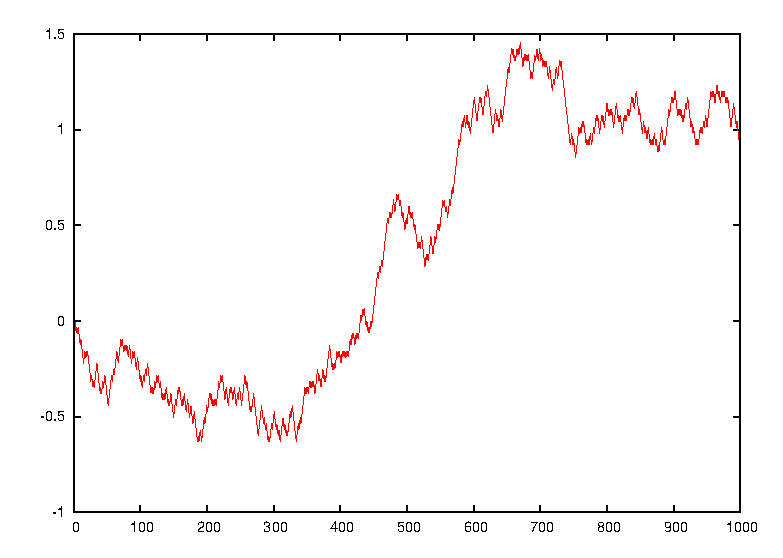
\includegraphics[width=10cm]{kikuchiBM_2.eps}
\]
\Subsubsection{確率積分}
確率積分とはブラウン運動に沿った積分のことです.
つまり,被積分関数と微小時間におけるブラウン運動の差分
をかけあわせたものを足しあげたものが確率積分です.
\footnote{これはざっくりとした説明です.数学的に厳密に
確率積分を構成するには確率論の知識が必要です.}
これは数理ファイナンスで言うと,ある時刻から他の時刻までの
利益を計算するときに使います.
確率積分は次のように書かれます.
\begin{equation*}
 X=\int_{0}^{T}f(t)dW(t).
\end{equation*}
また,これは直感的な理解がしやすいように微分形で書かれることもあります.
\begin{equation*}
 dX=fdW.
\end{equation*}
\Subsubsection{伊藤の公式と伊藤過程}
次は伊藤の公式と呼ばれているもので,通常の微積分で言うと
合成関数の微分公式にあたります.
\[
 df(t,W(t))=\frac{\D f}{\D t}dt+\frac{\D f}{\D x}dW+
 \frac{1}{2}\frac{\D^2f}{\D x^2}dt.
\]
これは,形式的に左辺をTaylor展開することによって,次のような
規則であると考えることもできます.
\begin{screen}
\begin{center}
 $dWdW=dt,\ dtdW=dWdt=0,\ dtdt=0.$
\end{center}
\end{screen}
また,次のような形を持つものを伊藤過程と言います.
\[
 dX(t)=\Delta (t)dW(t)+\theta (t)dt.
\]
伊藤過程についての積分を次のように定義します.
\[
 \int_{0}^{T}\Gamma (t)dX(t)=\int_{0}^{T}\Gamma(t)\Delta(t)dW(t)
 +\int_{0}^{T}\Gamma(t)\theta(t)dt.
\]
伊藤過程についても伊藤の公式が成り立ちます.
\begin{eqnarray*}
 df& = &\frac{\D f}{\D t}dt+\frac{\D f}{\D x}dX
 +\frac{1}{2}\frac{\D^2f}{\D t^2}dtdt+\frac{\D^2f}{\D t\D x}dtdX
 +\frac{1}{2}\frac{\D^2f}{\D x^2}dXdX\\
 & = &\frac{\D f}{\D t}dt+\frac{\D f}{\D x}\Delta dW 
 +\frac{\D f}{\D x}\theta dt+
 \frac{1}{2}\frac{\D^2 f}{\D x^2}\Delta^2dt.\\ 
\end{eqnarray*}
\kikueg 幾何ブラウン運動
\\
定数$\alpha$と$\sigma$に対して,
\[
 X(t)=\int_{0}^{t}\sigma dW(s)+
 \int_{0}^{t}\left(\alpha-\frac{1}{2}\sigma^2\right)ds
\]
とおきます.
また,定数$S(0)$と$f(x)=S(0)\exp x$に対して
\[
 S(t)=f(X(t))
\]
を幾何ブラウン運動と言います.
実は,幾何ブラウン運動は1期間二項モデルを多期間にして,
極限を取ると現れます.
\\
伊藤の公式によって次が成り立ちます.
\begin{eqnarray*}
 dS(t)& = &df(X(t))\\
 & = &\frac{\D f}{\D x}dX(t)+\frac{1}{2}\frac{\D^2f}{\D x^2}dXdX \\
 & = &S(t)dX(t)+\frac{1}{2}S(t)\sigma^2dt \\
 & = &\alpha S(t)dt+\sigma S(t)dW(t).
\end{eqnarray*}
\Section{\S 5.Black-Scholesモデル}
それではファイナンスの話題に戻りましょう.
ここでは最もスタンダードなBlack-Scholesモデルを考えます.
このモデルは,1種類の株式と1種類の銀行預金が存在する市場について
分析します.
$S(t)$を時刻$t$での株価とします.ここでは,$S(t)$は幾何ブラウン運動
に従うものとします.
\[
 dS(t)=\alpha S(t)dt+\sigma S(t)dW(t).
\]
また,金利は$r>0$とします.
次に,$X(t)$を時刻$t$でのポートフォリオの価値とします.
すると,$X(t)$は次の確率微分方程式を満たします.
\[
 dX(t)=\Delta(t)dS(t)+r(X(t)-\Delta(t)S(t))dt
\]
ただし,$\Delta(t)$は時刻$t$での株式保有数とします.
この式は,右辺の第1項が株式への投資額,第2項が銀行預金の額
の微小時間における差分を表しています.
$dS(t)$に幾何ブラウン運動を代入して計算を進めると,
\[
 dX(t)=rX(t)dt+\Delta(t)(\alpha-r)S(t)dt+\Delta(t)\sigma S(t)dW(t)
\]
となります.
ここで,$c(t,x)$を時刻$t$,株価$x$でのヨーロピアンコールオプションの
価格とします.
すると,伊藤の公式より,
\begin{eqnarray*}
 dc(t,S(t))& = &\frac{\D c}{\D t}dt+\frac{\D c}{\D x}dS+
  \frac{1}{2}\frac{\D^2c}{\D x^2}dSdS\\
 & = &\frac{\D c}{\D t}dt+
  \frac{\D c}{\D x}\left(\alpha S(t)dt+\sigma S(t)dW(t)\right)+
  \frac{1}{2}\sigma^2S^2\frac{\D^2c}{\D x^2}dt\\
 & = &\left(\frac{\D c}{\D t}+\alpha S(t)\frac{\D c}{\D x}+
  \frac{1}{2}\sigma^2S^2\frac{\D^2c}{\D x^2}\right)dt+
  \sigma S\frac{\D c}{\D x}dW
\end{eqnarray*}
となります.
したがって,ポートフォリオ$X(t)$でヨーロピアンコールオプションを
複製するためには,
\[
 X(0)=c(0,S(0)),\ dX(t)=dc(t,S(t))
\]
となれば良いので,$dW$の項を比較して
\[
 \Delta(t)=\frac{\D c}{\D x}(t,S(t)),
\]
$dt$の項を比較して,
\begin{eqnarray*}
 rX(t)& = &rc(t,S(t)) \\
 & = &\frac{\D c}{\D t}(t,S(t))+rS(t)\frac{\D c}{\D x}(t,S(t))+
  \frac{1}{2}\sigma^2S^2(t)\frac{\D^2c}{\D x^2}(t,S(t))
\end{eqnarray*}
となります.最初の式は,株式保有数は右辺のようにすればよい
ということを示しています.これはデルタヘッジと呼ばれます.
また,第2式から
\[
 rc(t,x)=\frac{\D c}{\D t}(t,x)+rx\frac{\D c}{\D x}(t,x)+
  \frac{1}{2}\sigma^2x^2\frac{\D^2c}{\D x^2}(t,x)
\]
と適当な境界条件
を満たす$c(t,x)$を見つければ良いことが分かります.
この偏微分方程式をBlack-Scholes方程式と言います.
\Section{\S 6.BS方程式を解く}
では,最後にBlack-Scholes方程式を解きましょう.
まずは,$y=\log x$と変数変換します.すると,
\begin{eqnarray*}
 \frac{\D}{\D x}& = &\frac{1}{x}\frac{\D}{\D y},\\
 \frac{\D^2}{\D x^2}& = &-\frac{1}{x^2}\frac{\D}{\D y}+\frac{1}{x^2}
  \frac{\D^2}{\D y^2}
\end{eqnarray*}
となります.また,$\tau = T - t$とすると,
\[
 \frac{\D}{\D t}=-\frac{\D}{\D\tau}
\]
となります.これらの変数変換によってBlack-Scholes方程式は
次のように変形できます.
\[
 -\frac{\D c}{\D\tau}+\left(r-\frac{1}{2}\sigma^2\right)
 \frac{\D c}{\D y}+\frac{1}{2}\sigma^2\frac{\D^2c}{\D y^2}-rc=0.
\]
次に,
\[
\begin{cases}
 \alpha=\frac{1}{2}-\frac{r}{\sigma^2}\\
 \beta=-\frac{1}{8\sigma^2}(\sigma^2+2r)^2
\end{cases}
\]
に対して,$c=\exp(\alpha y+\beta\tau)U$
とすると,
\[
 -\frac{\D U}{\D\tau}+\frac{1}{2}\sigma^2\frac{\D^2U}{\D y^2}=0
\]
となります.
ここで,$\tau$を改めて$\frac{1}{2}\tau\sigma^2$とすると,
\[
 \frac{\D U}{\D\tau}=\frac{\D^2U}{\D y^2}
\]
となります.
これは,熱伝導を記述する熱方程式というものになっています.
このように変形して数値計算すると,$c(t,x)$は次のような形になることが
分かります.\footnote{Black-Scholes方程式は解析解を持ちますが,
長くなるのでここでは省略します.}
ただし,実線はペイオフを表し,点が数値計算により
得られたヨーロピアンコールオプションの価格を示しています.
\[
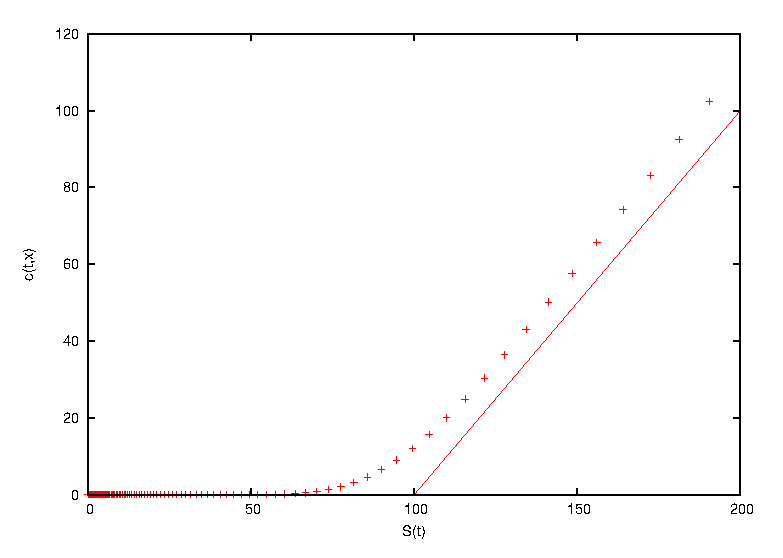
\includegraphics[width = 10cm]{kikuchiBS.eps}
\]
%\begin{thebibliography}{9}
% \bibitem
% \bibitem 
%\end{thebibliography}

\Section{参考文献}
\begin{description}
\item{[1]} Steven E. Shreve,``Stochastic Caluculus for Finance II  Continuous-Time Models'',Springer
\item{[2]} 関根順,``数理ファイナンス'',培風館
\end{description}
\Chapter{あなたにも(間違いが)分かるフェルマーの定理不完全証明(笠浦)}
%\Section{あなたにも(間違いが)分かるフェルマーの定理不完全証明(笠浦)}
\Section{\S 0. はじめに}

厳密な論証のみを主張の根拠とする数学の分野においては,「トンデモ」とよばれるものは存在しないと思われがちだが,実はそうでは無い.

長年数学雑誌の編集に携わってきた亀井哲治郎氏によると,「フェルマーの定理」や「四色問題」といった有名な数学の問題を「解いた」という投書が後を絶たないのだという.当然それらの「証明」が数学雑誌に掲載されることはないため,彼らがいかなる誤りを犯していたのかは知るよしもない.しかし中には,自身の「証明」の出版にまでこぎつけたアマチュア数学者もいる.

この記事ではそうした例の一つを紹介する.

あるとき私は,東大駒場図書館の数学書の棚に,数論の教科書に交じって「あなたも解けるフェルマーの定理完全証明」という本が置かれているのを見つけた.

フェルマーの定理とは,$n\geq 3$のとき方程式
\[a^n+b^n=c^n\]
は自然数解を持たないという主張である.

17世紀の数学者フェルマーが本の余白にこの式を書き込んで以後,三百年以上もの間,多くの数学者が証明に取り組み,ついに1995年にアンドリュー・ワイルズによって完全な証明がなされた.(証明までの経緯はサイモン・シンによるドキュメンタリー「フェルマーの最終定理」に詳しく書かれている.)

ワイルズによる証明は極めて専門的かつ長大であるので,「あなたにも解ける」とはどういうことかと中身を覗いてみたところ,案の定「アレな本」であった.こんな本を開架においておく駒場図書館もどうかと思ったが,これはきっと「情報の正しさを自分で判断するリテラシーを身につけてほしい」という司書さんからのメッセージだと判断し,「証明」の検証を行うことにした.

\Section{\S 1. 証明は驚くほどたやすかった}

小野田襄二著「あなたにも解けるフェルマーの定理完全証明」(めいけい出版 2003年)は300ページほどの本だが,6部構成になっており,定理の証明自体は最初の20ページほどを占める第1部「フェルマーの定理の証明I」で済んでいる.残りの第2部~第6部はその解説や別証明に充てられている.第1部の扉には(証明は驚くほどたやすかった)と書かれており,なるほど人類を三百年以上も悩ましてきた難問がなんの前準備もなく20ページで解けるならば驚くべきことだろう.

第1部の扉の文言をさらに引用すると,

\begin{quotation}
ビックリ玉手箱の蓋を開けたら【証明の王子】がささやいた\\

2003年4月17日のことでした.【証明の王子様】がささやいてくれたのです.それはそれは,驚くほど簡単で,喉から手が出るほど欲していたものでした.【証明の王子様】のしめくくりのことばを紹介します.
\begin{center}
\textbf{【人間の英知】のために人類に贈り物を捧げよう.}
\end{center}
\end{quotation}

ユーモアのつもりなのかもしれないが,完全に危ない人である.\textbf{玉手箱の蓋を開けてはいけない.}

それでは小野田氏による証明を見ていこう.なお,この本の文章はところどころわかりにくいところがあり,わたしが読み取れた範囲で論理を組み立てなおしている部分があることをお断りしておく.変数名や括弧の付け方は小野田氏のオリジナルに従った.

まずフェルマーの方程式
\[a^n+b^n=c^n\]
の両辺を$a,b,c$の最大公約数で割り,$a,b,c$はそれぞれ互いに素としてよいことを示している.ここまでは普通である.つぎに「$n=3$の証明によって,$n\geq 3$のすべてを証明してくれる」と主張して$n=3$の場合の証明に移っている.


\Subsubsection{$n=3$のときの証明 矛盾とその解消}

小野田氏はまず,
\[b^3=c^3-a^3=P\]
とおき,この式を\textcircled{\scriptsize 1}としている.さらに
\[c^3-a^3=b\cdot b^2\]
と変形し,この式を\textcircled{\scriptsize 2}としている.さきほどとほとんど変わらない式なのでわざわざ\textcircled{\scriptsize 2}とおく必要もない気がするが,まあいいだろう.

\textcircled{\scriptsize 2}の左辺を因数分解して,
\[(c-a)(c^2+ca+a^2)=b\cdot b^2\]
とし,さらに$(c-a)^2 \neq c^2+ca+a^2$であることから,
\[(c-a)\neq b\]
\[(c^2+ca+c^2)\neq b^2\]
を導いている.ここまではよい.

ところがこの式が書いてある部分の小見出しは「\textbf{★ \textcircled{\scriptsize 1}と\textcircled{\scriptsize 2}は矛盾を引き起こす}」である.べつに$(c-a)(c^2+ca+a^2)=b\cdot b^2$と上の式とは矛盾していない.これはどういうことなのだろうか?

さらにこの3ページ後,「\textbf{★ \textcircled{\scriptsize 1}と\textcircled{\scriptsize 2}との矛盾をクリアーする}」という謎の小見出しが登場する.「矛盾をクリアー」するとはどういうことなのだろう.

「矛盾をクリアーする」という節の内容を読んでみると,

\begin{quote}
最初の因数分解
\begin{eqnarray*}
(c^3-a^3)&=&b\cdot b^2\\
(c^3-a^3)&=&(c-a)(c^2+ca+a^2)
\end{eqnarray*}
が引き起こした矛盾は,素数の要素が二つ以上あることを念頭に入れていなかったからである.つまり,素数の要素が一つのときは,互いに素な二つの因数,$(c-a)$と$(c^2+ca+a^2)$に$b^3$を分けられない,あまりに当たり前のことを語っていただけのことである.
\end{quote}

要するに,「\textbf{$b$が素数の時しか考えてなかったから矛盾したような気がしたけど,よく考えたらそんなことなかったぜテヘペロ}」ということらしい.しかし読者としては,小野田氏が$b$が素数の場合しか考えてなかったことなど知る由もないし,こんな初歩的な混乱に読者をつき合わせる必要がどこにあるのだろう.

さらに言うと,$(c-a)\neq b$という式は今後使わない.なんのための議論だったのか.


\Subsubsection{$n=3$のときの証明 つづき}

気を取り直して先に進もう.
小野田氏によると,$a,c$は互いに素であることから,$(c-a)$と$(c^2+ca+c^2)$の最大公約数は1か3である.$c^2+ca+a^2=(c-a)^2+3ca$なのでこれは正しい.このことから小野田氏は

\begin{itemize}
\item $(c-a)$と$(c^2+ca+a^2)$が互いに素なとき,
\begin{eqnarray*}
(c-a)&=&(b_1)^3\\
(c^2+ca+a^2)&=&(b_2)^3\\
b&=&b_1b_2
\end{eqnarray*}

\item $(c-a)$と$(c^2+ca+a^2)$の最大公約数が3のとき,
\begin{eqnarray*}
(c-a)&=&3(b_1)^3\\
(c^2+ca+a^2)&=&3^{3q-1}(b_2)^3\\
b&=&3^qb_1b_2
\end{eqnarray*}
または,
\begin{eqnarray*}
(c-a)&=&3^{3q-1}(b_1)^3\\
(c^2+ca+a^2)&=&3(b_2)^3\\
b&=&3^qb_1b_2
\end{eqnarray*}
\end{itemize}

と場合分けする.二番目の場合分けは実際には不要だが,ここまではいい.
問題はそのあとの節である.

小野田氏は,第一の場合の二番目の式
\[(c^2+ca+a^2)=(b_2)^3\]
の左辺を因数分解して,
\[(c^2+ca+a^2)=(c-\sqrt{ca}+a)(c+\sqrt{ca}+a)\]
とする.$ca$が平方数でなければ,右辺の因数は整数にはならない.ここで小野田氏は奇妙な主張をする.

\begin{quote}
$\sqrt{ca}$が整数でなければ(無理数ならば),$(c^2+ac+a^2)$は,$1\cdot (c^2+ca+a^2)$を除いて,整数の積で表せないことを意味する.
\end{quote}

\textbf{意味するとは思えない.}小野田氏の主張によれば,$a,c$がいくつかの条件を満たしさえすれば$(c^2+ca+a^2)$は必ず素数になることになるが,そんなに簡単に素数が作れたら大変である.実際,$a=3,c=5$とでも置いてみれば$c^2+ca+a^2=49=7^2$となるが,$ca=15$は平方数ではない.どうして意味すると思ったのかよくわからない.

この主張は完全に誤りであるが,これを認めてしまえば証明はすぐそこである.

$(b_2)^3$は素数ではないので,$ca$は平方数で,$a,c$は互いに素なので$a=A^2,c=C^2$と書ける.すると
\[(C^2+CA+A^2)(C^2-CA+A^2)=(b_2)^3\]

ここで$A$と$C$は互いに素であることから,$(C^2+CA+A^2)$と$(C^2-CA+A^2)$も互いに素であることが導かれる.このことから,
\begin{eqnarray*}
(C^2+CA+B^2)&=&(B_1)^3\\
(C^2-CA+B^2)&=&(B_2)^3\\
\end{eqnarray*}
と書ける.

ここで,
\begin{eqnarray*}
(C^2+CA+B^2)&=&(C-\sqrt{CA}+A)(C+\sqrt{CA}+A)\\
(C^2-CA+B^2)&=&(C-\sqrt{3CA}+A)(C+\sqrt{3CA}+A)\\
\end{eqnarray*}
を用いれば,先ほどと同様の(破綻した)論法により$CA$と$3CA$はともに平方数となるが,これは$\sqrt{3}$が無理数であることに矛盾する.証明終了.

先ほどの場合分けの第二,第三の場合も本質的には同じである.


\Subsubsection{証明の問題点}
上記の証明の問題点は,そもそも論理が破綻しているというのもあるのだが,$(c-a)=(b_1)^3$という条件を使わず,$(c^2+ca+a^2)=(b_2)^3$という式のみから矛盾を導こうとしていることである.小野田氏は「★$\mathbf{(c^2+ca+a^2)=(b_2)^3}$\textbf{の条件吟味が全てだ}」と小見出しで宣言しているが,これはまずい.なぜなら$(c^2+ca+a^2)=(b_2)^3$には

\begin{eqnarray*}
1^2+1\cdot 18+ 18^2&=&7^3\\
17^2+17\cdot 36+ 36^2&=&13^3\\
17^2+17\cdot 73+ 73^2&=&19^3
\end{eqnarray*}
などの解があるし,$(c^2+ca+a^2)=3(b_2)^3$のほうも,
\begin{eqnarray*}
17^2+17\cdot 20+ 20^2&=&3\cdot 7^3\\
19^2+19\cdot 70+ 70^2&=&3\cdot 13^3
\end{eqnarray*}
などの解がある.

したがって第一の条件を無視し第二の条件に的を絞った小野田氏の方針は,失敗が宿命づけられていたといえる.

\Subsubsection{$n\geq 3$のときの証明}
$n=3$のときの証明ですでに破綻しているが,それ以上に気になるのは$n$が一般の場合に拡張できないことである.「$n=3$の証明によって,$n\geq 3$のすべてを証明してくれる」とはなんだったのか.

「$n\geq 3$のときの証明」の章は次のように始まっている.

\begin{quotation}
\[b^n=c^n-a^n\]
において,$b^n$の約数$b^{n-1},b^{n-2},\dots b^2$に対応する$(c^n-a^n)$の約数が存在するためには
\[c^n-a^n=(c-a)(c+a)^{n-1}\]
で表されなければならない.
\end{quotation}

\textbf{なぜだ.}どうしてそうなるのかわたしには全く分からない.

$c^n-a^n=(c-a)(c+a)^{n-1}$が成り立つのは$n=2$のときのみだ,だから$n\geq 3$のときは自然数解は存在しない,証明終了,となっているが,証明になっていないだけでなく,$n=3$のときの証明ともつながっていない.


実は「$n=3$のときの証明」の章の最後で小野田氏は,$(c^2+ca+a^2)=(b_2)^3$の左辺が$(c^2+2ca+c^2)$か$(c^2-2ca+a^2)$だったら,$(c+a)^2$や$(c-a)^2$と因数分解できるので無数の整数解を簡単に見つけられることを指摘している.それはそうなのだが,しかしそのことがこの式にどうつながるのだろうか? なんにせよ飛躍が多すぎて証明になっていない.


\Subsubsection{第二の証明}
この本の第四部は「フェルマーの定理の証明II」と題されており,第1部とは別の「証明」が書かれている.この証明は「第1部の証明を知ってしまった今となっては,まことに色あせたもの」らしく,なるほど第1部より長く,さらに読みづらい.

しかしどうも第1部と同種の誤りを犯しているようである.
まず,$(c^2+ca+a^2)^{\frac{1}{3}}$が整数になりえないことを示す,という間違った方針をとっている.
\[L=(c^2+ca+a^2)^{\frac{1}{3}}\]
とおき,$M=c+a$とおいてこれを
\[ca=M^2-L^3\]
と変形する.ここまではいい,しかしこのあと,$M^2-L^3$の「因数分解」として
\[M^2-L^3=(M^{\frac{2}{3}}-L)(M^{\frac{4}{3}}+M^{\frac{2}{3}}L+L^2)\]
および
\[M^2-L^3=(M-L^{\frac{3}{2}})(M+L^{\frac{3}{2}})\]
なる計算を行い,左辺が合成数なので,右辺の因数が整数になると考えてしまっているようである.もちろん実際にはこれらが整数になるとは限らない.

\Subsubsection{まとめ}

どうして小野田氏はこのような奇妙な「証明」を行ってしまったのだろう.

どうも小野田氏は,式として因数分解できるということと,その式に値を入れた結果が因数分解できるということを混同しているように思える.たしかに式として因数分解できれば値を入れても(因数の値が$\pm 1$にならなければ)因数分解されることになるが,逆は成り立たない.たとえば$f(X)=X$という多項式はもちろん既約だが,$X=6$を代入すれば$f(6)=6$となり素数にはならない.

そのうえで,中途半端に無理式を考慮している.$(c^2+ca+a^2)$を無理式の積で表すなら,
\[(c^2+ca+a^2)=(c+\sqrt{3ca+3a^2}+2a)(c-\sqrt{3ca+3a^2}+2a)\]
でもよいはずなのだが,なぜ上記の$\sqrt{ca}$が出てくる式だけ考えるのかよくわからない.

\Section{\S 2. 数学王国}

証明の検討はこれくらいにして,この本のほかの部分を拾い読みしてみよう.

まず本を開くと,目次より先に「社主激白」としてめいけい出版社長の言葉が載っている.「激白」とあるので出版の裏事情の暴露でもするのかと思ったら,小野田氏に対する狂わんばかりの賞賛の言葉が並んでいる.特に印象的なのが次の文句だ.

\begin{quote}
いま,社主が夢みることは,小野田氏を核に集う数学大好き人間が打ち立てる数学王国の実現である.危機の日本を救うのは数学立国の建設を措いてない.小野田氏の魅惑的なプランはもう次々と仕掛けられている.日本の未来は明るく輝いてきた.ひとなつこい小野田氏の輝く笑顔を見ると,だれでもこの人とともに,数学王国の建設に着手したい明るい気持ちになってくる.
\end{quote}

どこまで本気なのかよくわからない文章だが,なんだか「日本シャンバラ化計画」みたいで恐ろしい.\\

第5部「証明への道のり」には,小野田氏の「証明」完成までの経緯が書かれてる.
それによると,「コンピュータのハードを開発している友人」に「小野田さん,フェルマーの定理を証明したら」と「挑発」されたのが発端らしい.\textbf{罪作りな友人である}.そのあとの記述.

\begin{quote}
友人の挑発に乗り,証明のイメージをつかむことはできたのだが,高校1年で数学を捨て,大学入学と同時に数学と完全に縁を切った私である.
\end{quote}

\textbf{やっぱりな},という感じである.小野田氏の証明文の妙な読みにくさは,数学の高等教育を受けていないためなのだろう.

そして小野田は「証明」を完成させると,「読売年鑑の人名事典を調べ,およそ20人に近い数学者に原稿を送った」とのこと.さらにどうも証明を改訂するたびに数人の数学者に原稿を送っていたらしい.そのうち織田孝幸教授と浪川幸彦教授からは否定的な返事をもらい,織田教授は親切にも Paul Ribenboim 著『13 Lectures on Fermat's Last Theorem』からの抜粋をコピーして送ってくださったらしい.しかし小野田氏は英語が読めず,それどころか$A^3+B^3+C^3=0$という式だけを見て「\textbf{何というセンスの無さ}」というコメントをしてる有様である.

また著者の友人である田吉隆夫教授とは膨大な量の手紙のやり取りをしているらしい.この本にはそのうちのいくつかが載っており,田吉教授はきわめて誠実な態度で著者の「証明」の不明瞭な点を指摘していることがわかる.\textbf{持つべきものは友達である.}


\Section{\S 3. おまけ そのほかの小野田襄二氏の本}

小野田襄二氏にはほかにもさまざまな著作があるらしいので,おまけとして最後に紹介しておく.

\begin{itemize}

\item 自然数解が存在する全構造の解明 (社会評論社)

今回紹介した本の続編らしい.\textbf{タイトルが壮大すぎる.}

\item 相対性理論の誤りを完全解剖する (小野田書店)

理系トンデモ本の王道(?)の相対性理論批判であり,『完全証明』のカバーに広告が載っている.面白いのは次の指摘だ.

\begin{quote}
動物の目は網膜に入った光に反応し,空間を伝播している光を見ているのではない.ゆえに,光の相対速度は観測できない.
\end{quote}

何を言っているのかよくわからないが,いままでの光速度の測定は人間が肉眼で行ってきたとでも思っているのだろうか.

\item やりなおし基礎数学 (ちくま新書)

小中学生向けの数学の本らしい.注目すべきはこれがちくま新書から出ていることである.\textbf{ブランド名にだまされてはいけない}.

\item 夫婦耐性実験 (小野田書店)

小説である.「父親・夫として破綻したゲオが,ノイローゼの駿台生を引きとることによって巻き起こす家族騒動物語」らしい.タイトルが面白い.\textbf{ちょっとよみたい.}
\end{itemize}


\Section{\S 4. おわりに}

この手の本を読むことはよい暇つぶしになるが,そんなことをする暇があったらまともな数学書を読みましょう.

\Chapter{ゼータ関数(田村)}
%\Section{ゼータ関数(田村)}
\Section{\S 0.はじめに}
ますらぼには数学が好きな高校生も来るということで,なるべく高校生にもわかるよう書いてみた.正則性など細かい条件をごまかしているが,多項式や$e^x$などの高校で出てきた関数の組み合わせなら大体成り立つと思っておけばいい.興味のある人は複素解析の本を読んでみるといいと思う.\\
さて,タイトルのゼータ関数とは
\[
\zeta(s)=\sum_{n=1}^\infty\frac{1}{n^s}=\frac{1}{1^s}+\frac{1}{2^s}+\cdots
\]
という関数で,リーマンの論文「与えられた数よりも小さな素数の個数について」\cite{Riemann}にも現れる重要な関数である.\\
具体的な値を挙げておくと次の通りである.
\begin{eqnarray*}
\zeta(2)=\frac{1}{1^2}+\frac{1}{2^2}+\cdots &=& \frac{\pi^2}{6}\\
\zeta(4)=\frac{1}{1^4}+\frac{1}{2^4}+\cdots &=& \frac{\pi^4}{90}\\
\zeta(6)=\frac{1}{1^6}+\frac{1}{2^6}+\cdots &=& \frac{\pi^6}{945}
\end{eqnarray*}
偶数ゼータに対しては,なぜ$\pi$が出てくるのかは不思議だが,上の様な値になることが知られている.\\
では次の式を見てどう思うだろうか.
\begin{eqnarray*}
\zeta(0)=1+1+\cdots &=& -\frac{1}{2}\\
\zeta(-1)=1+2+\cdots &=& -\frac{1}{12}
\end{eqnarray*}
中辺は明らかに発散する無限和である.それが有限の値になるというのは理解し難い.少しずつその謎を紐解いていこうと思う.

\Section{\S 1.予備知識}
\Subsubsection{初等関数の複素数での値}
オイラーの公式$e^{iz}=\cos z+i\sin z$を用いると
\[
\cos z=\frac{e^{iz}+e^{-iz}}{2}, \sin z=\frac{e^{iz}-e^{-iz}}{2i}
\]
となる.\\
また,絶対値が$r>0$,偏角が$\theta$の複素数は$z=r(\cos\theta+i\sin\theta)=re^{i\theta}$となるので, $z$の対数は
\[
\log z=\log r +i\theta
\]
となる.ただし,偏角は$2\pi$の整数倍だけ異なることができるので, $\log$は一般には多価関数となる.そこで定義域を0と負の実数を除く領域に制限し,偏角を$-\pi<\theta<\pi$とすることで一価に定まる.これを対数関数の主枝と呼ぶ.

\Subsubsection{複素数平面上の積分}
$f(z)$が連続, $\gamma(t)\colon[0,1]\to\mathbb{C}$が区分的$C^1$であれば, $f(z)$の$\gamma$に沿った積分は
\[
\int_\gamma f(z)dz = \int_0^1 f(\gamma(t))\gamma'(t)dt
\]
となる.\\

\begin{wrapfigure}[7]{r}{50mm}
\vspace{-2\baselineskip}
\begin{center}
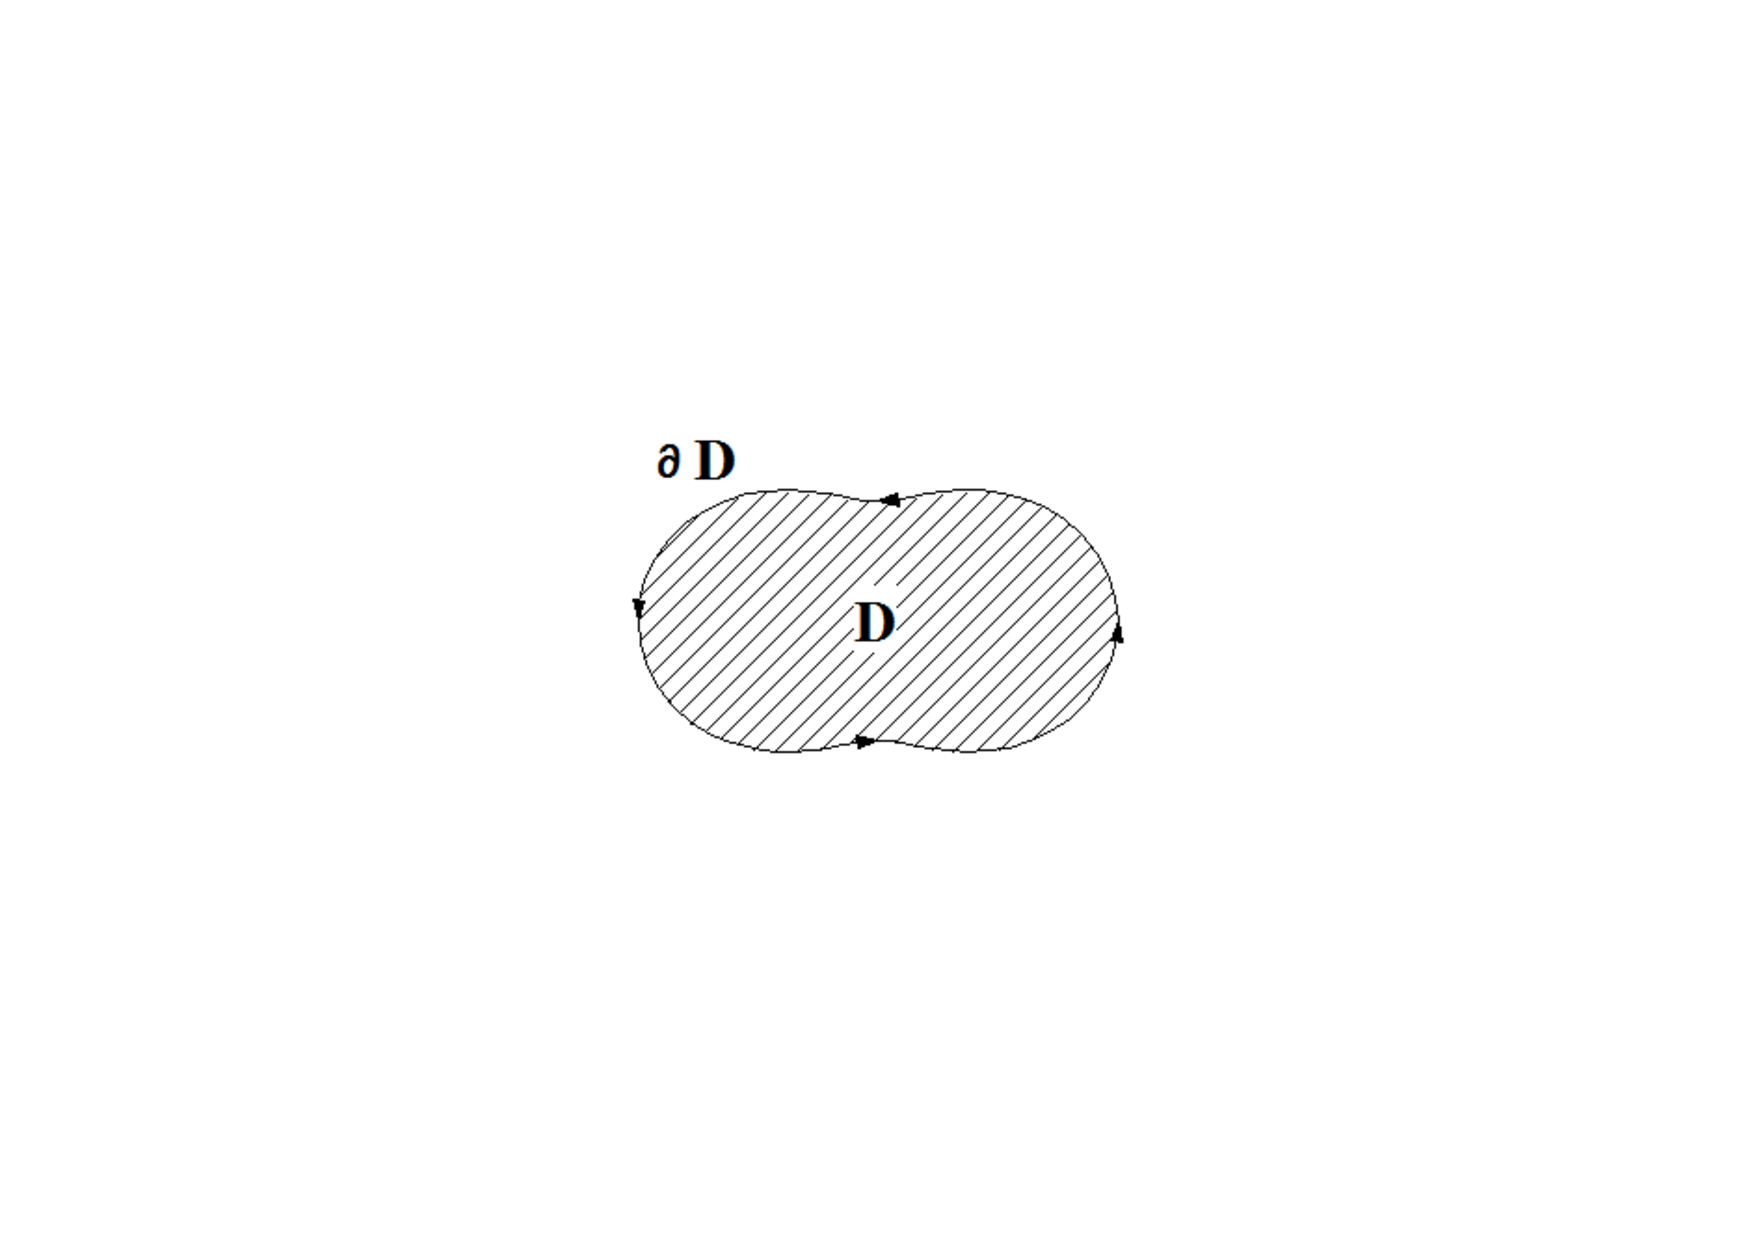
\includegraphics[width=50mm]{zetamura1.pdf}
\end{center}
\end{wrapfigure}
$D$を複素数平面上の区分的$C^1$の境界をもつ領域とし, $\partial D$を$D$の境界で$D$を左手に見て進む向きをもつ閉曲線とする.このとき次の公式が成り立つ.\\
$s\in \mathbb{Z}$とする. $a\in D$のとき
\begin{eqnarray*}
\frac{1}{2\pi i}\int_{\partial D} \frac{dz}{(z-a)^s} = \begin{cases}
1 & s=1 \\ 
0 & s\neq1
\end{cases}
\end{eqnarray*}
正則関数$f(z)$に対し$\displaystyle{\lim_{z\to a}f(z)}$が発散し, $\displaystyle{\lim_{z\to a}(z-a)^m f(z)}$が0以外の値に収束するとき, $z=a$を$f(z)$の$m$位の極という.\\
$f(z)$が$D$内に1位の極$z=a_n\,(n=1,2,\cdots)$をもち, $\displaystyle{\lim_{z\to a_n}(z-a_n)f(z)}=b_n$とすると次が成り立つ
\begin{eqnarray*}
\frac{1}{2\pi i}\int_{\partial D} f(z)dz = \sum_n b_n
\end{eqnarray*}

\Section{\S 2.$\zeta(s)$の解析接続}
リーマンは$\zeta(s)$について,1以外の全ての複素数sについて成り立つ式を求めた.\\
それは$Re(s)>1$をはみ出した領域での値を求めることであり
\[
\Pi(s-1)=\int_0^\infty e^{-x}x^{s-1}dx
\]
から始まる.この関数は$s$が正の整数の時$(s-1)!$に等しい関数である.\\
$x$を$nx$に置き換えると
\begin{eqnarray*}
\Pi(s-1) &=& \int_0^\infty e^{-nx}(nx)^{s-1}ndx\\
&=& n^s \int_0^\infty e^{-nx}x^{s-1}dx\\
\frac{\Pi(s-1)}{n^s} &=& \int_0^\infty e^{-nx}x^{s-1}dx
\end{eqnarray*}
両辺の和をとり
\begin{align}
\Pi(s-1)\zeta(s)=\int_0^\infty \frac{x^{s-1}dx}{e^x-1}\label{eq:1}
\end{align}
が求まる.\\

\begin{wrapfigure}[8]{r}{50mm}
\begin{center}
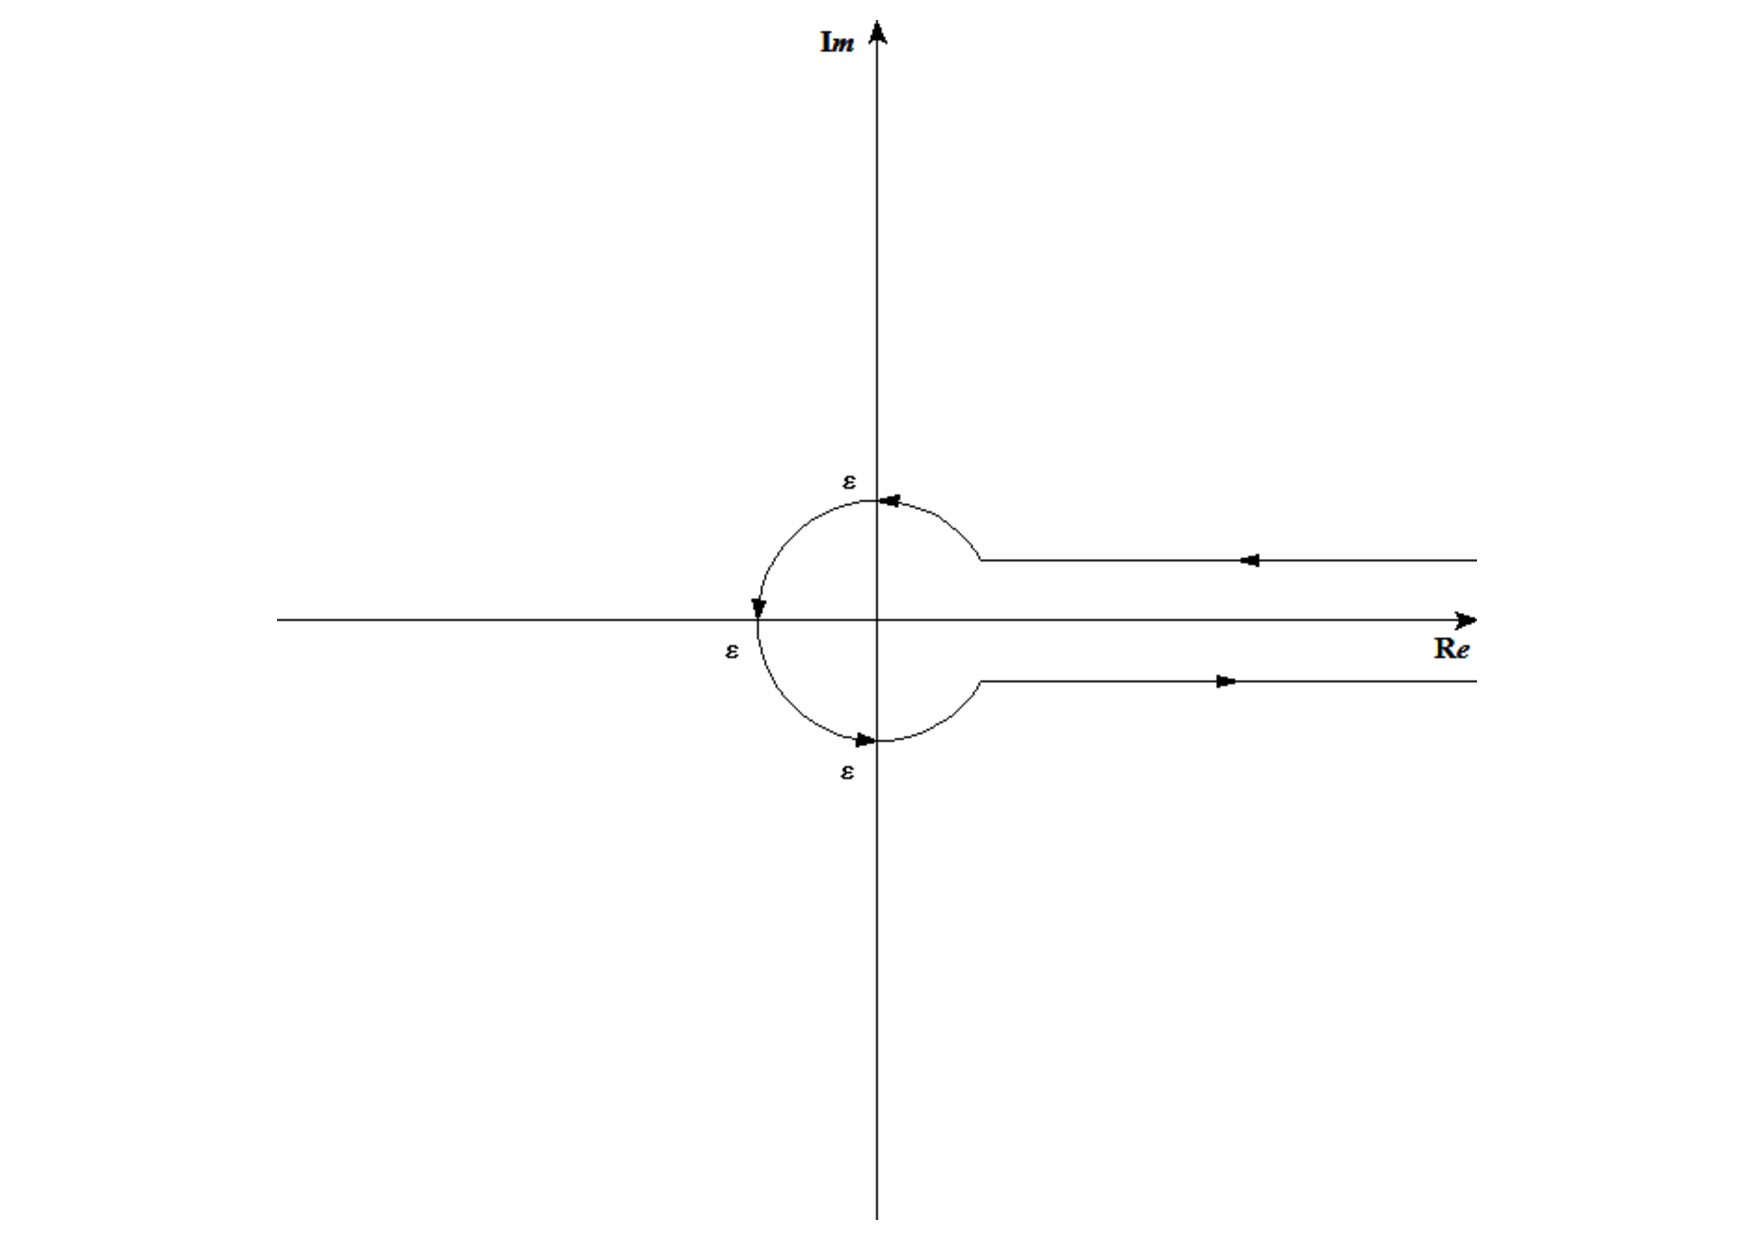
\includegraphics[width=50mm]{zetamura2.pdf}
\end{center}
\end{wrapfigure}
ここで以下の積分を考える.
\[
\int_{\infty}^{\infty} \frac{(-z)^{s-1}dz}{e^z-1}
\]
積分経路は,実軸よりわずかに上を通って$\infty$から0へと向かい, 0の周りを回ったのち,実軸のわずかに下を通って0から$\infty$へと向かう.\\
ただし, $(-z)^{s-1}=e^{(s-1)\log(-z)}$とし, $\log z$は主枝を選ぶ.\\

この積分を
\begin{align}
\int_{\infty}^\epsilon \frac{(-z)^{s-1}dz}{e^z-1}+\int_{|z|=\epsilon} \frac{(-z)^{s-1}dz}{e^z-1}+\int_\epsilon^{\infty} \frac{(-z)^{s-1}dz}{e^z-1}\label{eq:2}
\end{align}
と分割すると,中央の項は$Re(s)>1$において$\epsilon\to0$のとき0に近づく.\\
なぜなら, $|z|=\epsilon$のとき$|e^z-1|>1-e^{-\epsilon}>0$より$\frac{1}{|e^z-1|}<\frac{1}{1-e^{-\epsilon}}$であるから
\begin{eqnarray*}
\left|\frac{(-z)^{s-1}}{e^z-1}\right| \le \frac{\epsilon^{Re(s)-1}}{1-e^{-\epsilon}}
\end{eqnarray*}
であり, $\epsilon\to0$のとき
\begin{eqnarray*}
\left|\int_{|z|=\epsilon} \frac{(-z)^{s-1}dz}{e^z-1}\right| &\le& 2\pi\epsilon \frac{\epsilon^{Re(s)-1}}{1-e^{-\epsilon}}\\
&=& 2\pi\frac{\epsilon}{1-e^{-\epsilon}}\epsilon^{Re(s)-1}\to0
\end{eqnarray*}
となるからである.\\
残った2つの項をまとめると
\begin{eqnarray*}
\lim_{\epsilon \to 0}\left(\int_{\infty}^\epsilon \frac{(-z)^{s-1}dz}{e^z-1}+\int_\epsilon^{\infty} \frac{(-z)^{s-1}dz}{e^z-1}\right) &=& \lim_{\epsilon \to 0}\left(\int_{\infty}^\epsilon \frac{e^{(s-1)(\log z-i\pi)}dz}{e^z-1}+\int_\epsilon^{\infty} \frac{e^{(s-1)(\log z+i\pi)}dz}{e^z-1}\right)\\
&=& (e^{-\pi si}-e^{\pi si}) \int_0^\infty \frac{z^{s-1}dz}{e^z-1}\\
&=& -2i\sin{\pi s}\int_0^\infty \frac{z^{s-1}dz}{e^z-1}
\end{eqnarray*}
これを式(\ref{eq:1})と合わせれば次を得る.
\[
-2i\sin{\pi s}\,\Pi(s-1)\zeta(s)=\int_\infty^\infty \frac{(-z)^{s-1}dz}{e^z-1}
\]
右辺の積分は全てのsに対して収束し,正則である.\\
\[
\Pi(s-1)\Pi(-s)=\frac{\pi}{\sin{\pi s}}
\]
を用いれば
\begin{align}
\zeta(s)=-\frac{\Pi(-s)}{2\pi i}\int_{\infty}^{\infty} \frac{(-z)^{s-1}dz}{e^z-1}\label{eq:3}
\end{align}
となる.この式は複素平面上における$s=1$を除いて解析的な関数$\zeta(s)$を定義し, $Re(s)>1$において$\sum n^{-s}$と一致する.\\

\Section{\S 3.関数等式}
\begin{wrapfigure}[8]{r}{50mm}
\vspace{-2\baselineskip}
\begin{center}
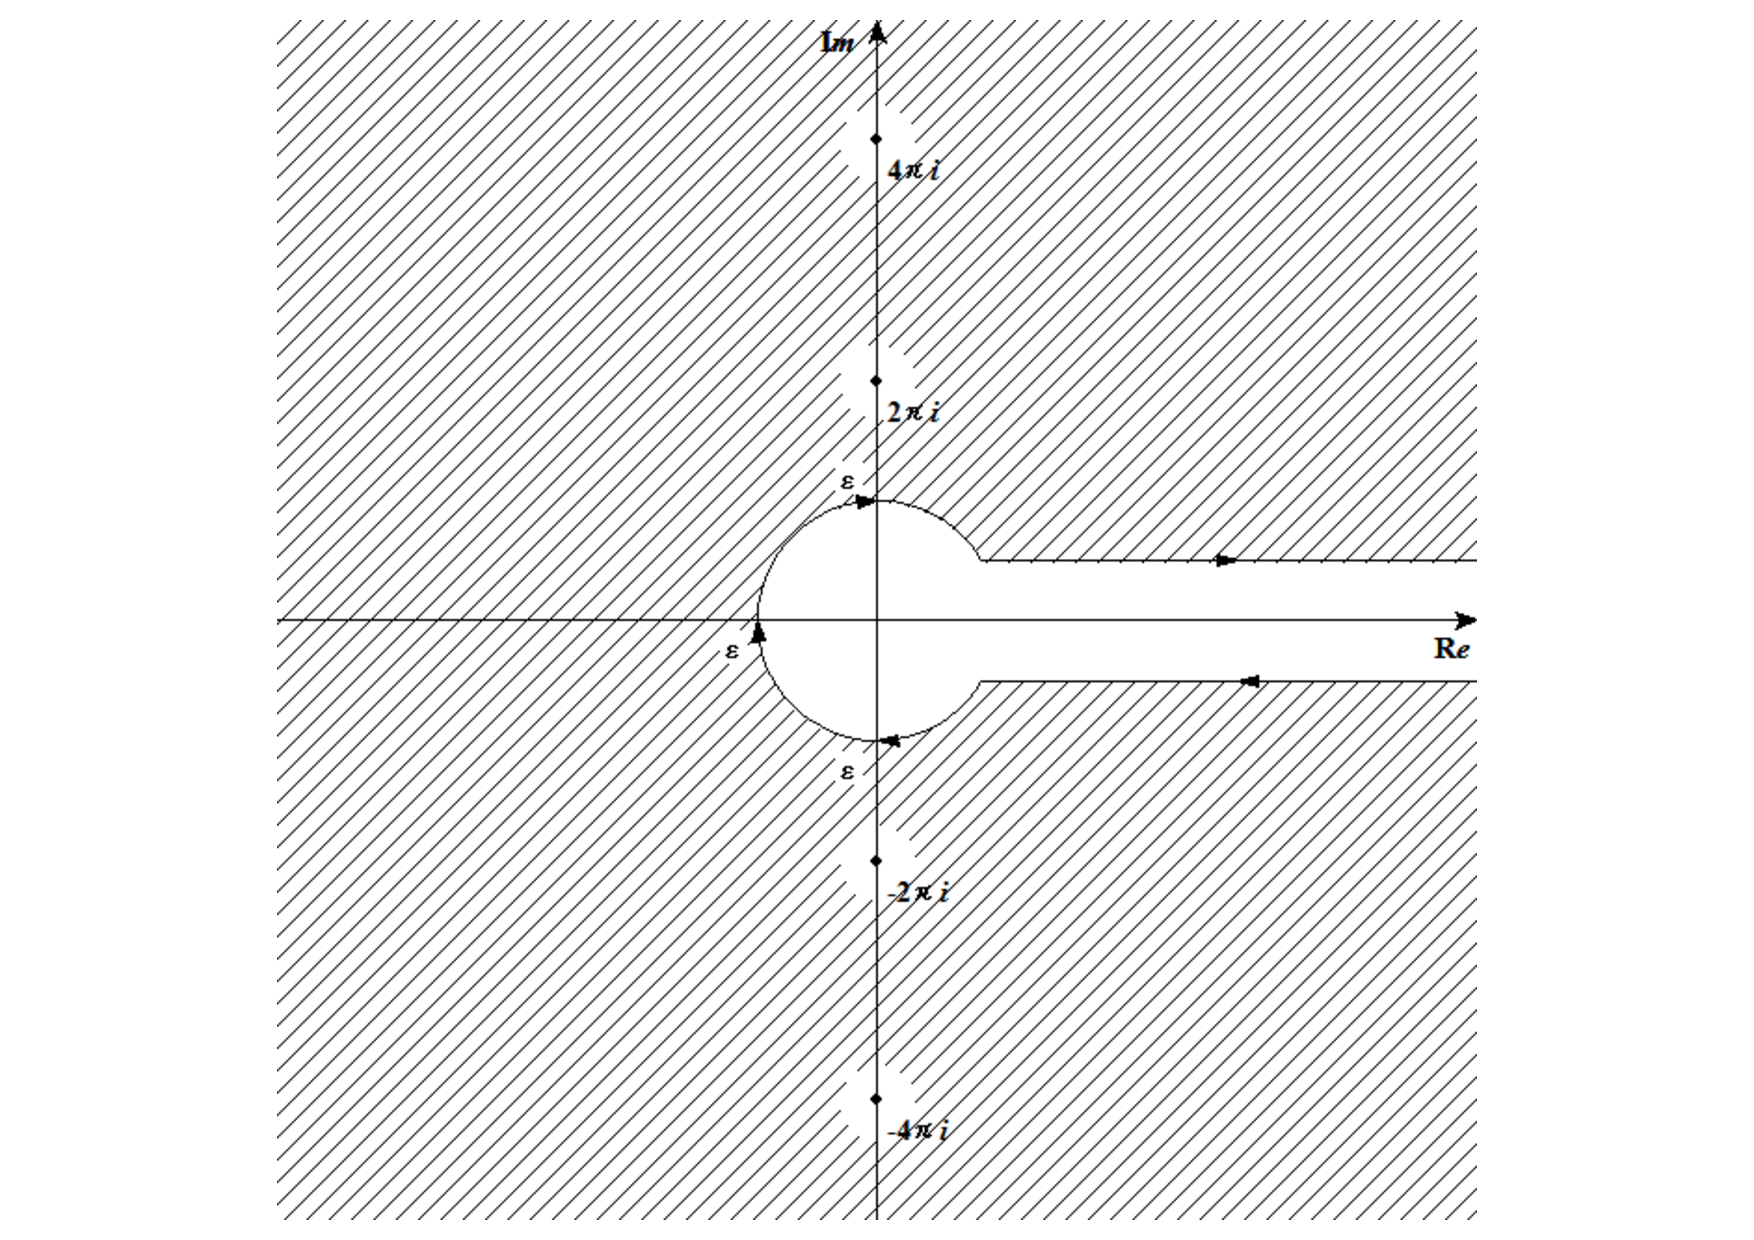
\includegraphics[width=50mm]{zetamura3.pdf}
\end{center}
\end{wrapfigure}
式(\ref{eq:3})において,積分経路を逆向きにとることで0以外の1位の極$z=2n\pi i\,(n=\pm1,\pm2,\cdots)$を含む領域に沿った積分とすることができる.値は$-1$倍になる事に注意して
\begin{eqnarray*}
\lim_{z\to 2n\pi i}(z-2n\pi i)\frac{(-z)^{s-1}}{e^z-1} &=& \lim_{z\to 2n\pi i}\frac{z-2n\pi i}{e^z-e^{2n\pi i}}(-z)^{s-1}\\
&=& (-2n\pi i)^{s-1}
\end{eqnarray*}
より
\begin{eqnarray}
\zeta(s) &=& \Pi(-s)\sum_{n=1}^\infty ((-2n\pi i)^{s-1}+(2n\pi i)^{s-1})\nonumber\\
&=& \Pi(-s)(2\pi)^{s-1}\left(i^{s-1}+(-i)^{s-1}\right)\sum_{n=1}^\infty n^{s-1}\nonumber\\
&=& \Pi(-s)(2\pi)^{s-1}2\sin\left(\frac{s\pi}{2}\right)\zeta(1-s)\label{eq:4}
\end{eqnarray}
が得られる.

\Section{\S 4.$\zeta(s)$の値}
さて, $\zeta(s)$の値をいくつか求めてみよう.\\
$s=-n\,(n\in\mathbb{N})$のとき,式(\ref{eq:3})より
\[
\zeta(-n) = -\frac{\Pi(n)}{2\pi i}\int_\infty^\infty \frac{(-z)^{-n-1}dz}{e^z-1}
\]
式(\ref{eq:2})と同様に分割すると,今度は第1項と第3項が打ち消し合い第2項のみが残るので
\begin{eqnarray*}
\zeta(-n) &=& -\frac{\Pi(n)}{2\pi i}\int_{|z|=\epsilon} \frac{(-z)^{-n-1}dz}{e^z-1}\\
&=& (-1)^n\frac{\Pi(n)}{2\pi i}\int_{|z|=\epsilon}\frac{z}{e^z-1}z^{-n-2}dz\\
&=& (-1)^n\frac{\Pi(n)}{2\pi i}\int_{|z|=\epsilon} \left(\sum_{m=0}^\infty \frac{B_m z^m}{m!}\right)z^{-n-2}dz\\
&=& (-1)^n \Pi(n)\sum_{m=1}^\infty \frac{B_m}{m!} \frac{1}{2\pi i}\int_{|z|=\epsilon} z^{m-n-2}dz\\
&=& (-1)^n n!\frac{B_{n+1}}{(n+1)!}\\
&=& (-1)^n \frac{B_{n+1}}{n+1}
\end{eqnarray*}

また, $n$を$2n-1$とすれば
\[
\zeta(-(2n-1))=(-1)^{2n-1}\frac{B_{2n}}{2n}
\]
となるが,関数等式(\ref{eq:4})を用いると
\[
\zeta(-(2n-1))=\Pi(2n-1)(2\pi)^{-2n}2\sin\left(\frac{-(2n-1)\pi}{2}\right)\zeta(2n)
\]
である.従って
\[
\zeta(2n)=(-1)^{n+1}\frac{(2\pi)^{2n}B_{2n}}{2(2n)!}
\]
を得る.\\
これらより最初に述べた式
\begin{eqnarray*}
\zeta(2)=\frac{\pi^2}{6}, \zeta(4)=\frac{\pi^4}{90}, \zeta(6)=\frac{\pi^6}{945}\\
\zeta(0)=-\frac{1}{2}, \zeta(-1)=-\frac{1}{12}
\end{eqnarray*}
等が求まるのである.

\Section{\S 5.解析接続の意味}
ゼータ関数を解析接続することで通常の和の意味では発散してしまう値を求めたわけでだが,これはどういう意味をもつのであろうか.\\
実は,例えば$Re s>-3$なるすべての複素数に対して
\[
\zeta(s)=\lim_{N\to\infty}\left\{\sum_{n=1}^N n^{-s}-\left(\frac{1}{1-s}N^{1-s}+\frac{1}{2}N^{-s}-\frac{s}{12}N^{-s-1}\right)\right\}
\]
となっている.\\
オイラーマクローリンの公式によれば
\[
\sum_{n=1}^N n^{-s}=\frac{1}{1-s}N^{1-s}+\frac{1}{2}N^{-s}-\frac{s}{12}N^{-s-1}+o(N^{-s-2})
\]
であるから,これと比較すればゼータ関数の解析接続は$\sum_{n=1}^N n^{-s}$の発散する部分を取り除いた和を求める,いわゆる繰り込みを行っているのである.従って最初に述べた
\begin{eqnarray*}
\zeta(0)=1+1+\cdots &=& -\frac{1}{2}\\
\zeta(-1)=1+2+\cdots &=& -\frac{1}{12}
\end{eqnarray*}
は正確ではなく,あくまで$\sum_{n=1}^\infty n^{-s}$を解析接続した関数$\zeta(s)$が$\zeta(0)=-\frac{1}{2},\zeta(-1)=-\frac{1}{12}$であると解釈する方が良いだろう.
\Section{参考文献}
\begin{description}
\item{[Harold]} ハロルド, M, E. 鈴木治郎訳(2012)『明解 ゼータ関数とリーマン予想』講談社
\item{[Kurokawa]} 黒川信重(2014)『ゼータの冒険と進化』現代数学社
\item{[Riemann]} Riemann, B. (1859). Ueber die anzahl der primzahlen unter einer gegebenen gr\"{o}sse. \textit{Monatsberichte der Berliner Akademie}, \textit{November 1859}, 671-680.
\end{description}

%\begin{thebibliography}{9}
%\bibitem{Harold}
%ハロルド, M, E. 鈴木治郎訳(2012)『明解 ゼータ関数とリーマン予想』講談社
%\bibitem{Kurokawa}
%黒川信重(2014)『ゼータの冒険と進化』現代数学社
%\bibitem{Riemann}
%Riemann, B. (1859). Ueber die anzahl der primzahlen unter einer gegebenen gr\"{o}sse. \textit{Monatsberichte der Berliner Akademie}, \textit{November 1859}, 671-680.
%\end{thebibliography}

%\Section{アーベル圏入門(鯖白(奴隷))}
\Chapter{アーベル圏入門(鯖白(奴隷))}
\Section{\S 1圏について}

\begin{defi}
圏$\mathcal{C}$は,
\begin{itemize}

\item 
{\bf 対象}(object)のクラス$\mathrm{Ob}(\mathcal{C})$.誤解の恐れがない時は$\mathrm{Ob}(\mathcal{C})$を単に$\mathcal{C}$と書く.
$X$が$\mathcal{C}$の対象であるとき,$X \in \mathrm{Ob}(\mathcal{C}) (または X \in \mathcal{C})$と書く.

\item 
任意の対象$X,Y$に対し{\bf $X$から$Y$への射}(arrow, morphism)の集合が存在する.
$\mathrm{Hom}_\mathcal{C}(X,Y)$で表す.
$f \in \mathrm{Hom}_\mathcal{C}(X,Y)$のとき,$X$は$f$の{\bf ドメイン},$Y$は$f$の{\bf コドメイン},と呼ぶ.
この$f$について,$f:X \to Y$,または$X \xrightarrow{f} Y$と書く.

\item 
任意の対象$X,Y,Z$に対し,$\mathrm{Hom}_\mathcal{C}(X,Y) \times \mathrm{Hom}_\mathcal{C}(Y,Z)$から$\mathrm{Hom}_\mathcal{C}(X,Z)$への写像が存在し,{\bf 合成}と呼ばれる.$(f,g)$の像は$g \circ f$または$gf$で表し,$f$と$g$の合成と呼ぶ.

\end{itemize}
以上から構成され,次の2つの条件を満たす.
\begin{itemize}
\item
$X \xrightarrow{f} Y \xrightarrow{g} Z \xrightarrow{h} W$のとき,$h \circ (g \circ f) = (h \circ g) \circ f$ (結合律)
\item
任意の対象$X$に対し{\bf 恒等射}(identity morphism) $\mathrm{id}_X \in \mathrm{Hom}_\mathcal{C}(X,X)$が存在し,任意の$f:X \to Y , g:Z \to X$に対し
\[
	f \circ \mathrm{id}_X = f, 	\mathrm{id}_X \circ g = g,
\]
が成り立つ.
\end{itemize}
\end{defi} \proofend

% \begin{defi}
%対象のクラスが集合である圏を{\bf 小圏}(small category)という.
%\end{defi} \proofend

\begin{ex}
集合の圏$\mathbf{Sets}$.対象は任意の集合であり,$X,Y \in \mathbf{Sets}$ に対し$\mathrm{Hom}_\mathbf{Sets}(X,Y)$は$X$から$Y$への写像全体,合成は通常の写像の合成である.
\end{ex} \proofend

\begin{ex}
アーベル群の圏$\mathbf{Ab}$.対象は任意のアーベル群であり,$X,Y \in \mathbf{Ab}$ に対し$\mathrm{Hom}_\mathbf{Ab}(X,Y)$は$X$から$Y$への準同型写像全体,合成は通常の写像の合成である.
\end{ex} \proofend

\begin{ex}
位相空間の圏$\mathbf{Top}$.対象は任意の位相空間であり,$X,Y \in \mathbf{Ab}$ に対し$\mathrm{Hom}_\mathbf{Top}(X,Y)$は$X$から$Y$への連続写像全体,合成は通常の写像の合成である.
\end{ex} \proofend

\begin{ex}
任意の半順序集合$C$は以下のようにすると圏$\mathcal(C)$とみなせる.

$\mathrm{Ob}(\mathcal{C}) = C$とし,$x, y \in C$に対し $x \leq y$のとき$\mathrm{Hom}_\mathcal{C}$は一元集合,$x \nleq y$のときは
$\mathrm{Hom}_\mathcal{C} = \emptyset$とする.このとき合成は推移律により定義でき,恒等射は反射律により存在する.

逆に,圏$\mathcal{C}$,$\mathrm{Ob}(\mathcal{C})$が集合であり,$X,Y \in \mathcal{C}$ に対し $\mathrm{Hom}_\mathcal{C}(X,Y)$が1元以上持たないならば,$\mathrm{Ob}(\mathcal{C})$は$X \leq Y \stackrel{\mathrm{def.}}{\Leftrightarrow} \mathrm{Hom}_\mathcal{C} \neq\emptyset$ と定めることにより半順序集合となる.
\end{ex} \proofend

\begin{ex}
任意のモノイド$M$は,1つのみの対象$e$を持つ圏$\mathcal{C}$と見ることができる.
実際$\mathrm{Ob}(\mathcal{C}) = {e},\mathrm{Hom}_{\mathcal{C}}(e,e) = M$とすると,$\mathcal{C}$は二項演算を合成として圏をなす.逆に1つのみの対象を持つ圏$\mathcal{C}$について,$\mathcal{C} = \{e\}$とすると$\mathrm{Hom}_{\mathcal{C}}(e,e)$は合成を二項演算としてモノイドになる.\\
特に群$G$は上のようにしてモノイドとみなせる.
\end{ex} \proofend

\begin{defi}
$\mathcal{C},\mathcal{C'}$を圏とする.$\mathcal{C'}が\mathcal{C}$の{\bf 部分圏}(subcategory)であるとは,
\begin{itemize}
\item $\mathrm{Ob}(\mathcal{C'}) \subset \mathrm{Ob}(\mathcal{C})$
\item 任意の$X,Y \in \mathcal{C'}$に対し $ \mathrm{Hom}(\mathcal{C'}) \subset \mathrm{Hom}(\mathcal{C})$
\item 任意の$X,Y, Z \in \mathcal{C'}, f:X \to Y , g:Y \to Z$ に対し,$g \circ f$が$\mathcal{C'}$と$\mathcal{C}$で一致する.
\item 任意の$X \in \mathcal{C'}$に対し$X$の恒等射が$\mathcal{C'}$と$\mathcal{C}$で一致する.
\end{itemize}
をみたすことである.\\
さらに$ \mathrm{Hom}(\mathcal{C'}) = \mathrm{Hom}(\mathcal{C})$を満たすとき,$\mathcal{C'}$は$\mathcal{C}$の{\bf 充満部分圏}(full subcategory)という.
\end{defi} \proofend

大雑把に,圏とは「ある構造を持つモノ(対象)とその間の写像など(射)を全体で考えよう」というものです.対象と射は,集合と写像のようなものですが,対象に関しては一般の圏では何らかの集合とは限らず,ただのラベルに過ぎません.射に関しても同じで,射は一般には集合から集合への写像とは限らず,ドメインとコドメインが指定されているだけです.ここで,一般の圏において写像の全射,単射に相当する概念を定義しよう.
\begin{defi}
$\mathcal{C}$を圏とする.\\
$m:Y \to Z$が{\bf mono}とは任意の$f,g:X \to Y$に対し,
\[ m \circ f = m \circ g  \; \Rightarrow \; f = g \]
が成り立つことである.\\
$e:X \to Y$が{\bf epi}とは任意の$f,g:Y \to Z$に対し,
\[ f \circ e = g \circ e \; \Rightarrow \; f = g \]
が成り立つことである.
\end{defi} \proofend

\begin{prop}
$f:X \to Y , g:Y \to Z$において,$g \circ f$がmonoならば$f$はmono,$g \circ f$がepiならば$f$はepiである.
\end{prop}
(証明)\;略\proofend

$\mathbf{Sets}$では$f$が単射であることとmonoであること,全射であることとepiであることは一致する.

\begin{defi}
$f: X \to Y , g: Y \to X$を圏$\mathcal{C}$の射とする.% $g \circ f = \mathrm{id}_X$であるとき,$f$は$g$の{\bf 右逆射},$g$は$f$の{\bf 左逆射}と呼ぶ.$f$に対し右逆射$g_r :Y \to X$と左逆射$g_l: Y \to X$が存在するとき,$g_l = g_l \circ \mathrm{id}_Y = g_l \circ (f \circ g_r) = (g_l \circ f )\circ g_r =\mathrm{id}_X \circ g_r$ より$g_r$と$g_l$は一致する.このとき$f$を{\bf 同型射}という.
$g \circ f = \mathrm{id}_X , f \circ g = \mathrm{id}_Y$が成り立つ時,$f,g$を{\bf 同型射}(isomorphism)という.このとき,XとYは{\bf 同型}(isomorphic)であるといい,$X \sim Y$で表す.
\end{defi} \proofend
$\mathbf{Sets}$ではmonoかつepiなら同型射ですが,一般には成り立たない.例えば$\mathbf{Top}$で,$X=\{0,1\}$に離散位相,密着位相を入れたものをそれぞれ$(X,\mathscr{O}_0),(X,\mathscr{O}_1)$とする.$\mathrm{id}_X : (X,\mathscr{O}_0) \to (X,\mathscr{O}_1)$はmonoかつepiだが,その逆写像は連続ではない.

\begin{defi}
$\mathcal{C}$を圏とする.$\mathcal{C}$の{\bf 始対象}(initial object)とは,対象$I \in \mathcal{C}$であり,任意の対象$X \in \mathcal{C}$に対し$I$から$X$へ唯一の射が存在するものである.$\mathcal{C}$の{\bf 終対象}(terminal object)とは,対象$T \in \mathcal{C}$であり,任意の対象$X \in \mathcal{C}$に対し$X$から$T$へ唯一の射が存在するものである.始対象かつ終対象である対象を{\bf ゼロ対象}と言う.
\end{defi} \proofend
始対象,終対象,ゼロ対象は存在すれば同型を除いて一意である.\\
$\mathbf{Sets}$において,空集合$\emptyset$は始対象で,任意の一元集合は終対象となる.$\mathbf{Sets}$にはゼロ対象は存在しない.$\mathbf{Ab}$において,自明な群$0 = \{e\}$は始対象かつ終対象,すなわちゼロ対象となる.

\begin{defi}
$\mathcal{C}$を圏,$A,B\in \mathcal{C}$とする.$A,B$の{\bf 直積}(product)とは対象$A \times B$であり,射$\pi_A : A \times B \to A , 
\pi_B : A \times B \to B$が存在し,任意の$X \in \mathcal{C}, f_A : X \to A , f_B: X \to B$に対し $f_A = \pi_A \circ f , f_B = \pi_B \circ f$
を満たす$f : X\to A \times B$が一意的に存在するようなものをいう(このような性質を直積の普遍性という).$A \prod B$とも書く.\\
\[
\xymatrix{
	& \ar[dl]_{f_A} X  \ar@{-->}[d]^{f}  \ar[dr]^{f_B}	& \\
A 	& \ar[l]^{\pi_A} A \times B \ar[r]_{\pi_B} 	& B 
}
\]
$A,B$の{\bf 直和}(coproduct)とは対象$A \bigoplus B$であり,射$\iota_A : A  \to A \bigoplus B, 
\iota_B : B \to  A \bigoplus B$が存在し,
任意の$X \in \mathcal{C}, f_A : A \to X , f_B: B \to X$に対し $f_A = f \circ \iota_A , f_B = f \circ \iota_B$
を満たす$f : A \bigoplus B \to X$が一意的に存在するようなものをいう(このような性質を直和の普遍性という).$A \coprod B$とも書く.\\
\[
\xymatrix{
	& \ar@{<-}[dl]_{f_A} X  \ar@{<--}[d]^{f}  \ar@{<-}[dr]^{f_B}	& \\
A \ar[r]_{\iota_A}	&  A \bigoplus B  & \ar[l]^{\iota_B} B 
}
\] 
\end{defi} \proofend

\begin{defi}
$\mathcal{C,D}$を圏とする.$\mathcal{C}$から$\mathcal{D}$への{\bf 関手}(functor)$F$とは
\begin{itemize}
\item 
$\mathrm{Ob}(\mathcal{C})$から$\mathrm{Ob}(\mathcal{D}$)への対応\\
 $\mathrm{Ob}(\mathcal{C}) \ni X \mapsto F(X) \in \mathrm{Ob}(\mathcal{D})$
 
 \item 
$X,Y \in \mathrm{Ob}(\mathcal{C})$,$\mathrm{Hom}_\mathcal{C}(X,Y) $から$\mathrm{Hom}_\mathcal{D}(F(X),F(Y))$への写像\\
$\mathrm{Hom}_\mathcal{C}(X,Y) \ni f \mapsto F(f) \in \mathrm{Hom}_\mathcal{D}(F(X),F(Y))$
\end{itemize}
 であって,以下を満たすものである.
 
 \begin{itemize}
 \item
 $X \in \mathcal{C}, \mathrm{id}_X \in \mathrm{Hom}_\mathcal{C}(X,X)$に対し$F(\mathrm{id}_X) = \mathrm{id}_{FX} \in \mathrm{Hom}_\mathcal{D}(FX,FX)$
 \item
 $X,Y,Z \in \mathcal{C}, X \xrightarrow{f} Y \xrightarrow{g} Z$に対し$F(g \circ f) = F(g) \circ F(f)$ \\
 $F(X),F(f)$を単に$FX,Ff$と書いたりもする.
  
 \end{itemize}
 写像$\mathrm{Hom}_\mathcal{C}(X,Y) \ni f \mapsto F(f) \in \mathrm{Hom}_\mathcal{D}(F(X),F(Y))$が全射のとき,Fを{\bf 充満関手}(full functor),単射のとき,{\bf 忠実関手}(faithful functor)という.
\end{defi} \proofend

%\begin{ex}
%関手の例?
%end{ex} \proofend

\begin{defi}
$\mathcal{C},\mathcal{D}$を圏.$F,G$を$\mathcal{C}$から$\mathcal{D}$への関手とする.$F$から$G$への{\bf 自然変換}$\eta$とは,各対象$X \in \mathcal{C}$に対して射$\eta_X : FX \to GX $が定まっていて,次の図式を可換にするようなものである.
\[ 
\xymatrix {
	FX	\ar[r]^{Ff} \ar[d]_{\eta_X}	& FY \ar[d]^{\eta_Y} \\
	GX	\ar[r]^{Gf} 				& GY
}
\]
\end{defi} \proofend

\Section{\S 2アーベル圏について}
\begin{defi}
圏$\mathcal{A}$が{\bf 加法圏}(additive category)であるとは,任意の$X,Y \in \mathcal{A}$に対し,$\mathrm{Hom}_\mathcal{A}(X,Y)$がアーベル群となり,かつ$\mathcal{A}$がゼロ対象$0$と,直積$X \times Y$(任意の$X,Y \in \mathcal{A}$) を持つことである.
\end{defi} \proofend
加法圏のモデルは加法群の圏$\mathbf{Ab}$である.$\mathbf{Ab}$は実際Hom集合はアーベル群となり,ゼロ対象$0 = {e}$を持ち,
アーベル群$G_1,G_2$に対して直積$G_1 \times G_2 $が存在するので,加法圏である.\\
加法圏$\mathcal{A}$において,対象$X$から$0$,$0$から$X$への唯一の射を同じ記号$0_X$で表す.に対し
$0 : X \to Y$を$0_{XY} = 0_Y \circ 0_X$とする.$\mathcal{A}$は加法圏より,$\mathrm{Hom}_\mathcal{A}(X,Y)$はアーベル群をなすが,その単位元は$0_XY$であることが容易に確かめられる. また,$f:W \to X , g:Y\to Z$ に対し$0_{XY} \circ f = 0_{WY} ,
g \circ 0_{XY} = 0_{XZ}$ もわかる.以下,$0_{XY}$などを単に0と書く.
\[
\xymatrix{
&	X \ar[r]^{0_{XY}} \ar@/_/[rrd]^{0_{XZ}}& Y \ar[dr]^{g} \\
W  \ar[ur]^f \ar@/_/[urr]_{0_{WY}}&&&Z
}
\]
$\mathbf{Ab}$において(圏論的)直積と(圏論的)直和は一致するが,実は一般の加法圏においてもこれが成り立つ.
\begin{prop}
加法圏$\mathcal{A}$の任意の対象$X,Y$に対し,直和$X \bigoplus Y$が存在し.直積と一致する.
\end{prop}
(証明)
$\mathrm{id}_X : X \to X, 0 :Y \to X$に対し,直積$X \times Y$の普遍性を用いると,
\[
\pi_X \circ \iota_X = \mathrm{id}_X\;\;\;\;\;\pi_Y \circ \iota_X = 0
\]
をみたす$\iota_X : X \to X\times Y$が一意的に存在する.
\[
\xymatrix{
	& \ar[dl]_{\mathrm{id}_X} X  \ar@{-->}[d]^{\iota_X}  \ar[dr]^{0}	& \\
X 	& \ar[l]^{\pi_X} X \times Y \ar[r]_{\pi_Y} 	& Y 
}
\]
同様にして,$0: Y \to X, \mathrm{id}_Y:Y \to Y$に対し,直積$X \times Y$の普遍性を用いると,
\[
\pi_X \circ \iota_Y = 0\;\;\;\;\;\pi_Y \circ \iota_Y = \mathrm{id}_Y
\]
をみたす$\iota_X : X \to X\times Y$が一意的に存在する.
\[
\xymatrix{
	& \ar[dl]_0 Y  \ar@{-->}[d]^{\iota_Y}  \ar[dr]^{\mathrm{id}_Y}	& \\
X 	& \ar[l]^{\pi_X} X \times Y \ar[r]_{\pi_Y} 	& Y 
}
\]
\\
さて,次の図式は上の$\iota,\pi$の式より可換である.
\[
\xymatrix{
	& \ar@/_/[dl]_0 X \times Y  \ar[d] | {\iota_X \circ \pi_X + \iota_Y \circ \pi_Y}  \ar@/^/[dr]^{\mathrm{id}_Y}	& \\
X 	& \ar[l]^{\pi_X} X \times Y \ar[r]_{\pi_Y} 	& Y 
}
\]
\\
また,上の$\iota_X \circ \pi_X + \iota_Y \circ \pi_Y$を$\mathrm{id}_{X \times Y}$に取り替えても可換である.直積の普遍性より,
上の図式を可換にする$X \times Y$から$X \times Y$への射は唯一なので,
\[
\iota_X \circ \pi_X + \iota_Y \circ \pi_Y = \mathrm{id}_{X \times Y}
\]
が成り立つ.
この$\iota_X,\iota_Y$が直和の普遍性を満たすことを示そう.\\
$Z\in \mathcal{A},f:X \to Z, g:Y \to Z$とする.$h : X \times Y \ o Z $を$h = f \circ \pi_X + g \circ \pi_Y$とすると,このhは下図を可換にする.
\[
\xymatrix{
& \ar@{<-}[dl]_f Z  \ar@{<-}[d]^{h}  \ar@{<-}[dr]^{g}  \\
X \ar[r]^{\iota_X} &  X \times Y & 	\ar[l]_{\iota_Y}  Y 
}
\]
\\
よって可換にするものの存在はいえた.このようなものが唯一であることをを示すために,$h_1,h_2: X \times Y \to Z $は
\[
h_1 \circ \iota_X = f \;\;\;\;\; h_1 \circ \iota_Y = g 
\]\[
h_2 \circ \iota_X = f \;\;\;\;\; h_2 \circ \iota_Y = g
\]
としよう.これより
\[
(h_1-h_2)\circ \iota_X = 0\;\;\;\;\;(h_1-h_2)\circ \iota_Y = 0
\]
となる,それぞれ右から$\pi_X,\pi_Y$を合成して和を取ると
\begin{align*}
0	&= (h_1 - h_2)\circ (\iota_X \circ \pi_X + \iota_Y \circ \pi_Y) \\
	&= (h_1 - h_2)\circ \mathrm{id}_{X \times Y} \\
	&= h_1 - h_2 
\end{align*}
より$h_1 = h_2$がわかる.
\proofend

さて,加法圏において,$\mathbf{Ab}$の準同型の核,像に相当するものを定義したい.しかしmono,epiのときと同様,対象は一般には集合ではないので,アーベル群と同じようには定義できない.まず,核,余核を,普遍性を使って定義する.

\begin{defi}
加法圏$\mathcal{A}$の射$f:X \to Y$の{\bf 核}とは,射$\mathrm{ker}(f): \mathrm{Ker}(f) \to X$で,$f \circ \mathrm{ker}(f) = 0$をみたし,次の普遍性を満たすものである. \\
{\rm(核の普遍性)}\;$k \circ f = 0$をみたす任意の$k:K \to X$に対し,下図を可換にする一意的な射$i:K \to \mathrm{Ker}(f)$が存在する.
\[
\xymatrix{
\mathrm{Ker}(f) \ar[r]^{\mathrm{ker}(f)} & X \ar[r]^f &Y  \\
K \ar[ur]_{k}  \ar@{.>}[u]^i
}
\]\\

また,加法圏$\mathcal{A}$の射$f:X \to Y$の{\bf 余核}とは,射$\mathrm{cok}(f): Y \to \mathrm{Cok}(f)$で,$\mathrm{cok}(f) \circ f = 0$をみたし,次の普遍性を満たすものである. \\
{\rm(余核の普遍性)}\;$f \circ c = 0$をみたす任意の$c:Y \to C'$に対し,下図を可換にする一意的な射$p:\mathrm{Cok}(f) \to C$が存在する.
\[
\xymatrix{
X \ar[r]^f 	& Y \ar[r]^{\mathrm{cok}(f)} &\mathrm{Cok}(f) \ar@{.>}[d]^p \\
&&C \ar@{<-}[ul]_{c}  
}
\]
\end{defi} \proofend
加法圏の核,余核は常に存在するとは限らない.対象より射の方に着目することが多いので,ここでは射の核,余核は射を指すことにする.$\mathrm{Ker}(f), \mathrm{Cok}(f)$は,2つあったら同型である.\\
$\mathbf{Ab}$の準同型$f:G_1 \to G_2$において包含写像$i:\mathrm{Ker}(f) \to G_1$は$f$の核であり,自然な全射$p:G_2 \to \mathrm{Cok}(f)$は$f$の余核である.

\begin{defi}
加法圏$\mathcal{A}$の射$f:X \to Y$の{\bf 像}とは,余核$\mathrm{cok}(f): Y \to \mathrm{Cok}(f)$の核$\mathrm{im}(f): \mathrm{Im}(f) \to Y$である.\\
また,加法圏$\mathcal{A}$の射$f:X \to Y$の{\bf 余像}とは,核$\mathrm{ker}(f): \mathrm{Ker}(f) \to X$の余核$\mathrm{coim}(f): X \to \mathrm{Coim}(f) $である.
\end{defi} \proofend
\begin{prop}
加法圏において,核はmonoであり,余核はepiである.
\end{prop}
(証明)\;略\proofend
\begin{prop}
加法圏$\mathcal{A}$の射$f:X \to Y$に対して
\begin{itemize}
\item $f$がmono $\Leftrightarrow f\circ e = 0$ならば$e=0$\;($e:W \to X$)
\item $f$がepi \;\;\;\;$\Leftrightarrow g\circ f = 0$ならば$g=0$\;($g:Y \to Z$)
\end{itemize}
\end{prop}
(証明)\;略\proofend

\begin{defi}
圏$\mathcal{A}$が{\bf アーベル圏}であるとは,$\mathcal{A}$が加法圏であり,任意の射$f$について
\begin{itemize}
\item 任意の射は核と余核をもつ.
\item 任意のmono射$m$はその余核の核である.つまり$m = \mathrm{ker}(\mathrm{cok(m)})$
\item 任意のepi射$e$はその核の余核である.つまり$e = \mathrm{cok}(\mathrm{ker(e)})$
\end{itemize}
をみたすことである.

\end{defi} \proofend

\begin{prop}
アーベル圏$\mathcal{A}$の射$f$は,monoかつepiならば同型射になる.
\end{prop}
(証明) $f$はmonoより$ f = \mathrm{ker}(\mathrm{cok}(f))$.$\mathrm{cok}(f) \circ f = 0 = 0 \circ f$.
$f$はepiなので$\mathrm{cok}(f) = 0$これより,$\mathrm{id}_Y:Y \to Y$は$0 = \mathrm{cok}(f)$の核になることがわかる.
核のコドメインは同型より,$f$は同型射となる.
\[
\xymatrix{
X \ar[rr]^{\mathrm{ker}(\mathrm{cok}(f))}_{f} | = && Y\ar[r]_{0}^{\mathrm{cok}(f)} | = & C  \\
&Y \ar@{-}[ul]^{\cong} \ar[ur]_{\mathrm{id}_Y}
}
\]
\proofend
アーベル圏$\mathcal{A}$の射$f : X \to Y$について,次の分解がある.
\[
\xymatrix{
&\mathrm{Im(f)} \ar[rd]^m  \\
X\ar[ru]^e \ar[rr]^f  && Y
}
\]
ここで,$m=\mathrm{im(f)}$である.この分解は,次のように得る.\\
余核の定義により$\mathrm{cok}(f) \circ f = 0$.$\mathrm{im}(f) = \mathrm{ker}(\mathrm{cok}(f))$なので,核の普遍性
より,下図を可換にする一意的な射$e: X \to \mathrm{Im}(f)$がのびる.
\[
\xymatrix{
&\mathrm{Im}(f) \ar[rd]^{\mathrm{im(f)}} \\
X\ar@{.>}[ru]^e \ar[rr]^f  && Y \ar[rd]^{\mathrm{cok}(f)} \\
&&& \mathrm{Cok}(f)
}
\]
$m=\mathrm{im(f)}$は核なのでmonoである.実は$e$がepiであることも示せる.
\begin{lem}
上の$f$に対し,mono射$m': K \to Y$と射$e': X \to K$について$f=m' \circ e'$が成り立つとき,次を可換にする一意的な射
$t :\mathrm{Im}(f) \to X$が存在する.
\[
\xymatrix{
X \ar[d]_{e'} \ar[r]^{e} & \mathrm{Im}(f) \ar[d]^m  \ar@{.>}[ld]_t\\
K \ar[r]_{m'} & Y
}
\]
\end{lem}
(証明) 
$p = \mathrm{cok}(m) ,\;p' = \mathrm{cok}(m')$とおく.$m$はmonoなので$m' = \mathrm{ker}(p')$.
$p'  m' = 0$より$p'  m'  e' = p'  f = 0$ .
よって$\mathrm{Cok}(f)$の普遍性より一意的な射$w : \mathrm{Cok}(f) \to C$が存在して
$p' = w p$.
\[
\xymatrix{
X \ar[d]_{e'} \ar[r]^e \ar[rd]^f 	& \mathrm{Im}(f)  \ar[d]^m  \\
K \ar[r]_{m'} 				& Y \ar[r]^{p'} \ar[d]_{p} &	C \\
						& \mathrm{Cok}(f) \ar@{.>}[ru]_w
}
\]
これより$p'  m = w  p  m = 0$.$m' = \mathrm{ker}(p')$なので,核の普遍性より
一意的な射$t:\mathrm{Im}(f) \to K$が存在して$m = m't$.これより右下の可換がいえた.
また$m'te = me = f = m'e'$.$m'$はmonoなので,$te = e'$.これより左上の可換が言えた.
\proofend

\begin{thm}
アーベル圏$\mathcal{A}$の射$f : X \to Y$の分解
\[
\xymatrix{
&\mathrm{Im(f)} \ar[rd]^m  \\
X\ar[ru]^e \ar[rr]^f  && Y
}
\]
において,$m$はmono,$e$はepiである.
\end{thm}
(証明)$m$は核なのでmonoである.$e$がepiを示す.射$r,s : \mathrm{Im(f)}  \to Z$で$re = se$をみたすとする.
$k = \mathrm{ker}(r-s)$とおく.核の普遍性より,下図を可換にする$e' : X \to \mathrm{Ker}(r-s)$が一意的に存在する.
\[
\xymatrix{
\mathrm{Ker}(r-s) \ar[rd]^k \\
&\mathrm{Im}(f) \ar@<1ex>^r[r] \ar@<-1ex>_s[r] & Z \\
X \ar@{.>}[uu]^{e'} \ar[ru]^e
}
\]
$k,m$はmonoよりその合成もmono.よって上の補題より,下図を可換にする一意的な射$t$が存在する.
\[
\xymatrix{
X \ar[d]_{e'} \ar[rr]^e && \mathrm{Im}(f) \ar[d]^m  \ar@{.>}[lld]_t\\
\mathrm{Ker}(r-s) \ar[r]_{k} & \mathrm{Im}(f)  \ar[r]_m& Y
}
\]
$m = m k t$で$m$はmonoより$kt=\mathrm{id}_{\mathrm{Im}(f)}$ .$k = \mathrm{ker}(r-s)$であったので
$(r-s)k = 0$.右から$t$を合成して$(r-s)kt=r -s = 0$.すなわち$r=s$.
\proofend

$\mathrm{Coim}(f)$を使っても同様の分解が得られる.monoとepi,核と余核は双対であるので,
上と同様に$f$はmono射$m$とepi射${\mathrm{coim}(f)}$によって分解されることが示される.
\[
\xymatrix{
&\mathrm{Coim(f)} \ar[rd]^{m}  \\
X\ar[ru]^{\mathrm{coim}(f)} \ar[rr]^f  && Y
}
\]
$\mathrm{Im(f)},\mathrm{Coim(f)} $による分解によって得られたepi射,mono射をそれぞれ$e,m$とする.
$\mathrm{Im(f)},\mathrm{Coim(f)} $の普遍性を使うと下図を可換にする$i:\mathrm{Im(f)} \to \mathrm{Coim(f)} $が一意的に存在する.

\[
\xymatrix{
&&\mathrm{Coim}(f)\ar[rrd]^m \ar[r]_i^{\cong}&\mathrm{Im}(f) \ar[rd]^{\mathrm{im}(f)} \\
&X\ar[ru]^{\mathrm{coim}(f)} \ar[rru]^e \ar[rrr]^f&&&Y \ar[rd]^{} \\
\mathrm{Ker}(f) \ar[ru]^{\mathrm{ker}(f)} &&&&& \mathrm{Cok}(f)
}
\]
$e = i \circ {\mathrm{coim}(f)}, m = {\mathrm{im}(f)} \circ i$なので$i$はmonoかつepi,したがって同型射である.よって次を得る.
\begin{thm}
アーベル圏$\mathcal{A}$の任意の射$f : X \to Y$に対し$\mathrm{Coim}(f) \cong \mathrm{Im}(f)$である.
\end{thm}
\proofend

\begin{defi}
アーベル圏$\mathcal{A}$の射の列$X \stackrel{f}{\to} Y \stackrel{g}{\to}Z$がYにおいて{\bf 完全}(exact)とは,
$\mathrm{im}(f) = \mathrm{ker}(f)$となることである. 
\end{defi} \proofend

\begin{defi}
$\mathcal{C}$を圏,$f:X \to Z, g:Y \to Z$を射とする.$f,g$の{\bf 引き戻し}(pullback)とは,下図の可換図式であり,以下の普遍性を満たすものである.
\[
\xymatrix
{
P \ar[r]^{q} \ar[d]^{p} 	& Y \ar[d]^g\\
X \ar[r]^{f}			& Z
}
\]
普遍性.$p' : P' \to Y, q': P' \to X$で$f \circ p' = g\circ q'$を満たすような$p',q'$に対し一意的な射$t:P' \to P$が存在し,下図を可換にする.
\[
\xymatrix
{
P' \ar@/_/[rdd]^{p'} \ar@/^/[rrd]^{q'}  \ar@{.>}[rd]^t\\
&	P \ar[d]^{p} \ar[r]^{q} 	& Y \ar[d]^g\\
&	X \ar[r]^{f}			& Z
}
\]
\end{defi} \proofend

\begin{defi}
$\mathcal{C}$を圏,$f:X \to Y, g:X \to Z$を射とする.$f,g$の{\bf 押し出し}(pushout)とは,下図の可換図式であり,以下の普遍性を満たすものである.
\[
\xymatrix
{
X \ar[r]^{g} \ar[d]^{f} 	& Z \ar[d]^q\\
Y \ar[r]^{p}			& P
}
\]
普遍性.$p' : Y \to P', q': Z \to P'$で$p' \circ f  =q' \circ g$を満たすような$p',q'$に対し一意的な射$t:P \to P'$が存在し,下図を可換にする.
\[
\xymatrix
{
X \ar[r]^{g} \ar[d]^{f} 	& Z \ar[d]^q\ar@/^/[rdd]^{q'}\\ 
Y \ar[r]^{p} \ar@/_/[rrd]^{p'}& P \ar@{.>}[rd]^t  \\
&&P'
}
\]
\end{defi} \proofend

上の対象$P$はどちらも同型を除いて一意である.

\begin{prop}
圏$\mathcal{C}$において,$f:X \to Z, g:Y \to Z$を射とし,
\[
\xymatrix
{
P \ar[d]^{p} \ar[r]^{q} 	& Y \ar[d]^g\\
X \ar[r]^{f}			& Z
}
\]
を引き戻しとする.このとき,$f$がmonoならば$p$もmonoである.
\end{prop}
(証明)$f$はmonoであるとする.$r,s:W \to P$を射とし,$pr=ps$であるとする.このとき$fpr = gqr = gqs = fps$.$f$はmonoなので$pr=qr$.これより引き戻しの普遍性から$r=s$がわかる.

\[
\xymatrix
{
W \ar@/^/@<1ex>[rrd]^{pr=ps} \ar@/_/@<-0.5ex>[rdd]_{qr=qs}  \ar@<0.5ex>[rd]^r\ar@<-1ex>[rd]_s\\
&	P \ar[d]^{p} \ar[r]^{q} 	& Y \ar[d]^g\\
&	X \ar[r]^{f}			& Z
}
\]
\proofend
アーベル圏ではepiの場合も成り立つ.
\begin{prop}
アーベル圏$\mathcal{A}$において,$f:X \to Z, g:Y \to Z$を射とし,
\[
\xymatrix
{
P \ar[r]^{q} \ar[d]^{p} 	& Y \ar[d]^g\\
X \ar[r]^{f}			& Z
}
\]
を引き戻しとする.このとき,$f$がepiならば$p$もepiである.
\end{prop}
(証明)
$f$はepiとする.直積$X \times Y$からZへの射$ f \pi_X - g  \pi_Y$の核を$m:P \to X \times Y$とすると,下図は引き戻しになる.
($m$が$f \pi_X - g  \pi_Y$の核であることから可換性がわかり,直積と核の普遍性により引き戻しの普遍性が導かれる.)
\[
\xymatrix
{
P \ar[r]^{\pi_Y m} \ar[d]_{\pi_X m} 	& Y \ar[d]^g\\
X \ar[r]^{f}			& Z
}
\]
上のPは同型を除いて一意であったので,上の図で$f$がepiならば$\pi_Y m$もepiを示せばよい.
このとき$f \pi_X - g  \pi_Y$はepiである.ある$h:W \to X \times Y$について$h(f \pi_X - g  \pi_Y) = 0$とする.命題16より
直積は直和でもあるので,$\iota_X$を合成すると
\[
	0 = h(f \pi_X - g  \pi_Y)\iota_X = hf \pi_X \iota_X =hf
\]
$f$はepiだったので$h=0$,よって$f \pi_X - g  \pi_Y$はepi.これより$f \pi_X - g  \pi_Y = \mathrm{cok}(m)$となる.
ある$v : Y \to V$について$v \pi_Y m=0$とする.$\mathrm{cok}(m)$の普遍性により
$v\pi_Y = v'(f \pi_X - g  \pi_Y)$をみたす$v' :V \to Z$が一意的に存在する.
\[
\xymatrix
{
P\ar[r]^m &X \times Y \ar[rd]_{f \pi_X - g  \pi_Y} \ar[r]^{v\pi_Y} & V \\
&&Z  \ar@{.>}[u]_{v'}
}
\]
$\iota_X$を右から合成すると,
$\pi_Y\iota_X=0$なので
\[
	0 = v\pi_Y\iota_X = v'(f \pi_X - g  \pi_Y)\iota_X = v'f\pi_X\iota_X =v'f
\]
$f$はepiなので$v'=0$,よって$v\pi_Y = 0$,$v= v\pi_Y\iota_Y=0$.
\proofend
\begin{cor}
アーベル圏において常に引き戻しが存在する.
\end{cor}
\proofend
\begin{prop}
アーベル圏$\mathcal{A}$において,$f:X \to Z, g:Y \to Z$の引き戻しを考える.$k=\mathrm{ker}(f)$とすると下図のような
一意的な分解$k = pk'$が得られ,$k'=\mathrm{ker}(q)$となる
\[
\xymatrix
{
								&P \ar[r]^{q} \ar[d]^{p} 	& Y \ar[d]^g\\
\mathrm{Ker}(f)\ar[r]^k \ar@{.>}[ru]^{k'}	&X \ar[r]^{f}			& Z
}
\]
\end{prop}
(証明)
$\mathrm{Ker}(f)$から$Y$へのゼロ射$0$を考えることにより,引き戻しの普遍性から一意的な射$k':\mathrm{Ker}(f)\to P$が
存在して$pk'=k,qk'=0$となる.
\[
\xymatrix
{
& K \ar@(l,u)@{.>}[ldd]_{u'} \ar[d]^{u}\\
&P \ar[r]^{q} \ar[d]^{p} 	& Y \ar[d]^g\\
\mathrm{Ker}(f)\ar[r]^k \ar@{.>}[ru]^{k'} &X \ar[r]^{f}			& Z
}
\]
この$k'$が$q$の核となることを示そう.$u:K \to P$を$qu=0$をみたす射とする.右から$g$を
合成すると$0=uqg = upf$となる.これより$\mathrm{Ker}(f)$の普遍性から一意的な射$u':K \to \mathrm{Ker}(f)$が存在して
$ku' = pu$.これにより引き戻しの普遍性が使えて,$u=k'u'$が導かれる.これより$k'$は$q$の核となる.
\[
\xymatrix
{
K \ar@/^/@<1ex>[rrd]^{0} \ar@/_/@<-0.5ex>[rdd]_{ku'=pu}  \ar@<0.5ex>[rd]^{k'u'}\ar@<-1ex>[rd]_{u}\\
&	P \ar[d]^{p} \ar[r]^{q} 	& Y \ar[d]^g\\
&	X \ar[r]^{f}			& Z
}
\]

\proofend
引き戻しについて上で示されたことの双対は,押し出しについても同様に示される.

\begin{defi}
アーベル圏$\mathcal{A}$の対象$X\in \mathcal{A}$をコドメインに持つ射$f$をXの{\bf メンバ}と呼び,$f \in {}_mX$で表す.
\end{defi} \proofend
$\mathcal{A}$をアーベル圏,$X\in \mathcal{A}$とする.Xのメンバ$f,g$について,あるepi射$u.v$が存在して$fu=gv$をみたすとき,
$f \equiv g$と定義する.明らかにこれは反射律,対称律をみたす. 推移律を確かめる.
\[
\xymatrix
{
\nkgr \ar[d]^{v'} \ar[r]^{w'} & \nkgr \ar[d]^v \ar[r]^u& \nkgr \ar[d]^f\\ 
\nkgr \ar[d]^r \ar[r]^w & \nkgr \ar[d]^g \ar[r]^g& \nkgr \\
\nkgr \ar[r]^h          & \nkgr
}
\]

$f \equiv g,g \equiv h$とすると,epi射$r,u,v,w$
が存在して$fu=gv,gw=hr$をみたす.下図において,$v,w$の引き戻しを考える.$v,w$epiなので命題29より$v',w'$もepi.よって$f \equiv z$である.
アーベル圏の任意の対象$X$について,$0 \in _mX$であり,$f \in _mX$なら$-f \in _mX$である.\\
$f:X \to Y$をアーベル圏の射とする.$p \in _mX$に対し$fp \in _mY$となる.$p,q \in _mX,p \equiv q$とすると$fp \equiv fq$となる.これより射$f$は,あたかも写像のようにXのメンバをYのメンバにうつす.
\begin{thm}
(図式追跡のための基本法則).アーベル圏におけるメンバについて,以下の性質が成り立つ.
\begin{enumerate}
\item $f:X \to Y $がmono $\Leftrightarrow$ 任意の$x \in _mX$に対し$fx \equiv 0$ならば$x\equiv0$
\item $f:X \to Y $がmono $\Leftrightarrow$ 任意の$x ,x' \in _mX$に対し$fx \equiv fx'$ならば$x\equiv x'$
\item $f:X \to Y $がepi $\Leftrightarrow$  任意の$y \in _mY$に対し$x \in _mX$が存在し$gx \equiv x$
\item $f:X \to Y $がゼロ射 $\Leftrightarrow$  任意の$x \in _mX$に対し$fx \equiv 0$
\item $\xymatrix@1{ X \ar[r]^f & Y \ar[r]^g & Z } $が$Y$で完全 $\Leftrightarrow$ $gf = 0$かつ$gy \equiv 0$を満たす$y \in _mY$に対し
$x \in _mX$が存在して$y \equiv fx$となる.
%\item これいるのかな?
\end{enumerate}
\end{thm}
(証明)\; 3.と5.だけ示す.\\
3.\; $f:X \to Y $をepi,$y \in _mY$とする. $f$と$y$に対し引き戻しを考える.
\[
\xymatrix{ \ar@{}[rd] |{p.b.}
\nkgr \ar[r]^e \ar[d]^x& \nkgr \ar[d]^y \\
X \ar[r]^f & Y
}
\]

このとき$f$はepiなので$e$もepi,よって$y \equiv fx$がわかる.

逆に$f$がepiでないとすると,どの$x\in _mX$に対しても$fx$はepiでないので,$fx \neq \mathrm{id}_Y \in {}_mY$である.


5.\; $\xymatrix@1{ X \ar[r]^f & Y \ar[r]^g & Z } $がYで完全とする.$\mathrm{Im}(f)$による$f$の分解$f = me$を考える.$Y$で完全より
$m=\mathrm{im}(f)=\mathrm{ker}(g)$.よって$gf = gme = g \mathrm{ker}(f) e = 0$.$y \in _mY$で,$gy \equiv 0$なものを考える.$\equiv$の定義から直ちに$gy = 0$がいえる.ここで,次の図式を考える.
\[
\xymatrix{
\nkgr \ar@{.>}[d]^{x}  \ar@{.>}[r]^{e'}& \nkgr \ar@{=}[r] \ar@{.>}^p[d]& \nkgr \ar[d]^y \\
X \ar[r]^e & \mathrm{Ker}(g) \ar[r]^m & Y
}
\]
核の普遍性から上を可換にする$p$が唯一存在する.$e,p$の引き戻しを上の図のように考えると$ye' = mex = fx$.
$e$はepiなので$e'$もepi.よって$x \in {}_mX$が存在して$y \equiv fx$となる.\\
逆に$gf = 0$かつ$gy \equiv 0$を満たす$y \in _mY$に対し$x \in _mX$が存在して$y \equiv fx$となるとする.$k = \mathrm{ker}(g)$は
$gk \equiv 0$を満たすので$x \in _mX$が存在して$k \equiv fx$.よって$ \mathrm{cok}(f) k \equiv \mathrm{cok}(f) fx \equiv 0 $なので
$ \mathrm{cok}(f) k = 0$.よって$\mathrm{Im}(f)$の普遍性から下図を可換にする射$p$が存在する.
\[
\xymatrix{
\nkgr \ar@{>>}[r] \ar@{>>}[d] & \mathrm{Ker}(g)\ar[rd]^k \ar@{.>}[r]^p & \mathrm{Im}(f) \ar[d]^{\mathrm{im}(f)}\\
\nkgr \ar[r]^x & X \ar[r]^f &Y \ar[d]^{\mathrm{cok}(f)} \ar[r]^g& Z \\
&&\mathrm{Cok}(f) 
}
\]
また$gf = 0$と$f$の分解$f = me$より$gf = gme = 0$.eはepiより$gm = 0$がわかる.よって$\mathrm{Ker}(g)$の普遍性から,下図を可換にする射$q$が存在する.
\[
\xymatrix{
&\mathrm{Im}(f)\ar[rd]^m \ar@{.>}[r]^	q&\mathrm{Ker}(g)\ar[d]^{\mathrm{ker}(g)} \\
X\ar[ru]^e \ar[rr]^f&&Y\ar[r]^g&Z
}
\]
この$p,q$に対して,$qp,pq$を考えると核と像の普遍性によりどちらも恒等射になる.これよりYで完全であることがわかった.
\proofend

この定理を用いると,アーベル圏における図式の補題が図式の追跡により示すことができる.

\begin{lem}五項補題(five lemma)\\
下図の可換図式
\[
\xymatrix{
X_1 \ar[d]^{f_1} \ar[r]^{g_1} & X_2 \ar[d]^{f_2} \ar[r]^{g_2} & X_3 \ar[d]^{f_3} \ar[r]^{g_3} & X_4 \ar[d]^{f_4} \ar[r]^{g_4} &
X_5 \ar[d]^{f_5}  \\
Y_1 \ar[r]^{h_1} & Y_1 \ar[r]^{h_2} & Y_3 \ar[r]^{h_3} & Y_4 \ar[r]^{h_4} & Y_5 
}
\]
において,行は完全であるとする.このとき,$f_1,f_2,f_4,f_5$が同型射ならば,$f_3$も同型射である.
\end{lem}
(証明)
$f_3$がmonoを示せば,双対的にepiも示されるので,$f_3$がmonoを示せば十分である.$x \in {}_mX$で$f_3x \equiv 0$とする.
これと図の可換から$f_4g_3x = h_4f_3x \equiv 0$.$f_4$はmonoなので$g_3x \equiv 0$.
完全性を用いて定理33の5.より$x_2 \in {}_mX$が存在して$x \equiv g_2x$.$h_2f_2x_2 \equiv f_3x \equiv 0 $.これより再び定理33の5.を用いると$y_1 \in {}_mY$が存在して$f_2x_2 \equiv h_1y_1$.$f_1$epiなので定理33の3.より$x_1\in {}_mX$が存在して$y_1 \equiv f_1x_1$.
$f_2g_1x_1 \equiv f_2x_2$と$f$:monoより$x_2 \equiv g_1x_1$.よって$x \equiv g_2g_1x_1 \equiv 0$.
\[
\xymatrix{
x_1\ar@{|.>}^{\mathrm{epi}}[d] & x_2 \ar@{|.>}[r] \ar@{|->}[d]&x \ar@{|->}[d] \ar@{|->}[r]& g_3x \ar@{|->}^{\mathrm{mono}}[d] \\
y_1 \ar@{|.>}[r]& f_2x_2 \ar@{|->}[r]& 0\ar@{|->}[r] & f_4g_3x
}
\]
\proofend
もうひとつ図式の補題を示すために,以下の列が完全である可換図式を考えよう.
\[
\xymatrix{
0 \ar[r] & X \ar[d]^f \ar[r]^m & Y \ar[d]^g \ar[r]^e & Z \ar[d]^h \ar[r] & 0 \\
0 \ar[r] & X' \ar[r]^{m'} &Y' \ar[r]^{e'} & Z' \ar[r] & 0 
}
\]
この図式で$f,g,h$の核,余核をとると,普遍性から以下の可換図式が得られ,一番上と一番下の行は完全である.
\[
\xymatrix{
0 \ar[r] & \mathrm{Ker}(f) \ar[d] \ar[r]^{m_0} &\mathrm{Ker}(g) \ar[d] \ar[r]^{e_0} & \mathrm{Ker}(h) \ar[d]   \\
0 \ar[r] & X \ar[d]^f \ar[r]^m & Y \ar[d]^g \ar[r]^e & Z \ar[d]^h \ar[r] & 0 \\
0 \ar[r] & X' \ar[d] \ar[r]^{m'} &Y' \ar[d] \ar[r]^{e'} & Z' \ar[d] \ar[r] & 0 \\
& \mathrm{Cok}(f) \ar[r]^{m_1} &\mathrm{Cok}(g) \ar[r]^{e_1} & \mathrm{Cok}(h) \ar[r] & 0  \\
}
\]
蛇の補題では上の完全列と下の完全列をつなぐ射の存在を示す.
\begin{lem}蛇の補題(snake lemma)\\
上の図式に対し,以下の列が完全になるような射$\delta:\mathrm{Ker}(h) \to \mathrm{Cok}(f)$が存在する.
\[
\xymatrix@1{
0 \ar[r] & \mathrm{Ker}(f)  \ar[r]^{m_0} &\mathrm{Ker}(g) \ar[r]^{e_0} & \mathrm{Ker}(h) \ar[r]^{\delta}
 & \mathrm{Cok}(f) \ar[r]^{m_1} &\mathrm{Cok}(g) \ar[r]^{e_1} & \mathrm{Cok}(h) \ar[r] & 0
}
\]
\end{lem}
(証明)
$K=\mathrm{Ker}(h),k=\mathrm{ker}(h),C=\mathrm{Cok}(f),c=\mathrm{cok}(f)$とする.$k$と$e$の引き戻し$u,k'$を取ると,
$e$はepiより$u$もepi.$m$の$S = \mathrm{Im}(f)$による分解を$m=pq$とすると,命題32より$s$による$p$の分解を得る.
($q$はmonoかつepiなので実は同型射である).下半分についても双対で同様のことを考える.下図はすべて可換になる.
\[
\xymatrix{
S \ar[rd]^p \ar@{.>}[r]^{s} &P \ar@{.>}[d]^{k'} \ar@{.>}[r]^{u} & K \ar[d]^k   \\
X \ar[u]^q_{\cong} \ar[d]^f \ar[r]^m & Y \ar[d]^g \ar[r]^e & Z \ar[d]^h  \\
X' \ar[d]^c \ar[r]^{m'} &Y' \ar[rd]^{q'} \ar@{.>}[d]^{c'} \ar[r]^{e'} & Z'    \\
C \ar@{.>}[r]^{v} &Q \ar@{.>}[r]^{t} & T \ar[u]_{p'}^{\cong} \\
}
\]
$\delta_0 = c'gk'$とする.$u=\mathrm{cok}(s)$かつ$v = \mathrm{ker}(t)$から$\delta_0$は一意的に
\[
\delta_0 = v\delta u : \xymatrix@1{P \ar[r]^u & K \ar[r]^{\delta} & C \ar[r]^v & Q}
\]
と分解できる.この$\delta$が求める射である.\\
メンバ$x \in {}_mK$から$\delta x \in {}_mC$は次の図式の追跡によって得られることを示そう.
\[
\xymatrix{
&&x \ar@{|->}[d] \\
&y \ar@{|->}[r] \ar@{|->}[d] &kx \ar@{|->}[d] \\
z \ar@{|->}[d] \ar@{|->}[r]   &gy \ar@{|->}[r] &0 \\
z_1
}
\] 
$e$はepiなので$y \in {}_mY$が存在して$ey \equiv kx$となる.$e'gy = hkx = 0$と,$Y'$での完全性から
$z \in {}_mX'$が存在して$gy \equiv m'z$.$z_1 = cz$とする.このとき$z_1 \equiv \delta x$となる.これを示そう.\\
まず$ey \equiv kx$と引き戻しの普遍性より,$x = ux_0,y = k'x_0$をみたすメンバ$x_0 \in {}_mP$が
一意的に存在することがわかる.
\[
\xymatrix
{
\nkgr \ar@/_/[rdd]_{y} \ar@/^/[rrd]^{x}  \ar@{.>}[rd]^{x_0}\\
&	P \ar[d]^{k'} \ar[r]^{u} 	& Y \ar[d]^k\\
&	X \ar[r]^{e}			& Z
}
\]
これより
\[
v\delta x \  v \delta ux_0 =\delta_0 x_0 = c'gy \equiv vz_1
\]
$v$はmonoより$\delta x \equiv z_1$となる.この式により,$z_1$の同値類は図式の追跡の際の
メンバの選び方に依存しないこともわかる.この追跡により,$\mathrm{Ker}(h),\mathrm{Cok}(f)$の完全性が示される.
(定理34を使う.頑張って!)
\proofend


\Section{参考文献}
\begin{description}
\item{[1]}S.マックレーン著,三好博之/高木理 訳,『圏論の基礎』,シュプリンガー・ジャパン,2012
\item{[2]}梶浦宏成著,『数物系のための圏論』,サイエンス社,2010
\item{[3]}Albercht Dold,``Lectures on Algebraic Topology'',Springer,1980(Reprint)
\item{[4]}Charles A. Weibel,``An introduction to homological algebra'',Cambridge University Press,1994
\end{description}


\Chapter{パズルのコーナー1.〜スリザーリンク〜(SP1)}
\Section{スリザーリンク}
\footnote{「スリザーリンク」「カックロ」の名称は(株)ニコリの登録商標です。}
\leavevmode \\
\\
\begin{figure}[h]
\centering
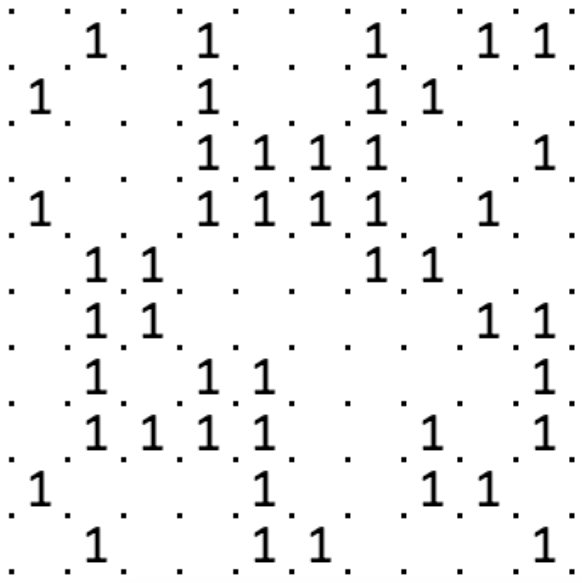
\includegraphics[width =7cm,bb = 0 0 202 202]{sp1slitherlink}
\end{figure}
\Subsection{スリザーリンクのルール}
\begin{description}
\item{1.} 点と点をタテヨコにつなげ、全体で1つの輪っかをつくります。
\item{2.}  4つの点で作られた小さな正方形の中の数字は、その正方形に引く辺の数です。数字のない小さな辺には、何本線を引くかは分かりません。
\item{3.} 線を交差させたり、枝分かれさせたりはしません。
\end{description}

¥Chapter{Counterexamples in Topology 傑作撰(宮本)}
¥Section{¥S 1.概説}
¥subsubsection*{反例の本}
数学は定理と証明を繰り返すだけではなかなか身につきにくく,適切な{¥bf 反例}を考えることで概念の有用性を理解できることが多い,というのは皆さん経験したことだと思います.歴史的にも,ワイエルシュトラスが連続かつ至るところ微分不可能な「病理的関数」を発見したことで,それまで「連続関数は大体のところで微分可能なんじゃないの〜?」と信じられていた雰囲気がぶち壊され,解析学が$¥varepsilon - ¥delta$論法による厳密化へと進展した.このようなことが度々あります.証明によって世界を広げていくというのが数学の基本だと思いますが,反例が「ある」という事実もまた心強いものです.¥par
今回は位相空間論の反例集である``¥textbf{Counterexamples in Topology}''  (Lynn Steen and J. Arthur Seebach, Jr)の内容から幾つか参考になりそうな例を紹介してみたいと思います.
¥subsubsection*{内容紹介}
本書は位相空間論の反例を大量に収録したある意味「病的な」本といえるかもしれませんが,学習の上で参照するにはうってつけの本だと思います.本書最大の特徴は,豊富なチャートにあります.例えば,正則であって正規でない位相空間を探そうと思ったら,分離公理について書かれた19ページの表を見て,反例90番が該当するということがすぐに分かります.定義間の主従関係が反例付きで載っていますし,巻末には各例について,どの公理を満たし,どの公理を満たさないかが網羅された表が掲載されており,検索に供するようになっています.¥par
第一部では位相の様々な定義(分離公理,コンパクト性,連結性,距離空間)を簡単に復習することができます.第二部がメインコンテンツの反例集で,143個の例が掲載されています.第三部は「位相空間はいつ距離空間になるか?」という距離化定理にまつわるサーベイとなっています(ここにも反例が載っています).付録の第四部では前述の網羅された表や演習問題,参考文献等が掲載されています.

¥Section{¥S 2.分離公理に関する反例}
¥subsubsection*{正則・正規}
まずは定義を簡単に復習しましょう.
¥begin{defi}[正則空間]
位相空間Xが{¥bf 正則}であるとは,以下の2つの条件をみたすことを言う.
¥begin{enumerate}
¥item $X$の任意の$1$点集合は閉集合である.
¥item $X$の任意の閉集合$A$と,$A$に含まれない任意の点$x$は開集合で分離される.すなわち,開集合$U$,$V$が存在して,$A¥subset U$,$x¥in V$かつ$U¥cap V=¥varnothing$が成立する.
¥end{enumerate}
¥end{defi}
¥begin{defi}[正規空間]
位相空間$X$が{¥bf 正規}であるとは,以下の2つの条件をみたすことを言う.
¥begin{enumerate}
¥item $X$の任意の$1$点集合は閉集合である.
¥item $X$の任意の交わらない閉集合の組$A,B$は開集合で分離される.すなわち,開集合$U$,$V$が存在して,$A¥subset U$,$B¥subset V$かつ$U¥cap V=¥varnothing$が成立する.
¥end{enumerate}
¥end{defi}
定義から明らかですが,正規性からは正則性が従います.また,距離空間は正規ですから,普通のユークリッド空間$¥mathbb{R}^n$は正規になります.正則であって,正規でない空間とはどのようなものでしょうか?
¥begin{ex}[Sorgenfrey空間]
$¥mathbb{R}$の開集合の基底を$U=[a,b)¥ (a,b¥in¥mathbb{R})$とした空間を$S$とする(Sorgenfrey直線).Sorgenfrey空間Xを$X=S¥times S$で定義する.
¥end{ex}
$X$での典型的な開集合は$[a,b)¥times[c,d)$という形をしており,これが$X$の開集合の基底になっています.ここで部分集合$¥Delta=¥{(x,-x)¥mid x¥in¥mathbb{R}¥}$を考えてみると,これは閉集合です.$¥Delta$内の任意の点$x$に対して$¥{ x ¥}$は誘導位相の下で開集合になるので,$¥Delta$に誘導される位相は離散位相となり,$¥Delta_1=¥{(x,-x)¥mid x¥in¥mathbb{Q}¥}$,$¥Delta_2=¥Delta¥setminus¥Delta_1$とすると,これらは$X$の閉集合です.ところが$¥Delta_1$を含む開集合と$¥Delta_2$を含む開集合は必ず交わってしまうことが示せるので$X$は正規ではありません.¥par
また,Sorgenfrey直線$S$は正則かつ正規であり,$2$つの正則空間の直積は正則なので$X$は正則です.このことから$X$が「正規空間の直積は正規」という命題の反例ということも分かりますね.¥par
 ¥par
正規空間は部分空間をとるという操作とも相性が悪く,正規空間の部分空間は正規とは限りません.
¥begin{defi}[全部分正規]
任意の部分空間が正規となるような正規空間$X$を{¥bf 全部分正規}であるという.
¥end{defi}
全部分正規でないような正規空間の例は,集合論的に少しむずかしい操作をして構成します.
¥begin{defi}
$¥omega$を最小の超限順序数(自然数の集合$¥mathbb{N}$に対応する順序数¥footnote{選択公理を認めさせてください.}),$¥Omega$を最小の非可算順序数とする.順序数には濃度の比較により全順序が入るので順序数$¥alpha,¥beta$に対して$[¥alpha,¥beta]=¥{x¥mid ¥alpha¥leq x¥leq ¥beta¥}$とする.
¥end{defi}
¥begin{ex}[Tychonoffの板]
$[0,¥omega]$,$[0,¥Omega]$にそれぞれ区間から定まる位相を入れ,$T=[0,¥omega]¥times[0,¥Omega]$とする..
¥end{ex}
順序数$¥alpha$に対して$[0,¥alpha]$に区間位相を入れた空間はコンパクトハウスドルフになり,その直積である$T$もコンパクトハウスドルフですから,コンパクトハウスドルフ空間が正規なことより$T$は正規空間です¥footnote{「$[0,¥alpha]$が正規だから,正規空間の直積である$T$も正規である」というのはダメですよね.}.¥par
ところが,$T$から$(¥omega,¥Omega)$という一点を除いた空間$T_{¥infty}$は正規で無くなってしまうのです.これは$T_{¥infty}$の部分空間$A=¥{(¥omega,¥alpha)¥mid 0¥leq ¥alpha<¥Omega¥}$,$B=¥{ (n,¥Omega)¥mid 0¥leq n<¥omega ¥}$が分離できない$2$つの閉集合であることを示すことで分かります.

¥subsubsection*{距離づけ可能定理と第二可算性}
位相空間というのは点同士の「近さ」が定義されている空間ですから,ある空間に「距離¥footnote{集合$X$上の距離とは以下の3つの公理を満たす$X$上の非負実数値関数$d$のことを言います.(i)$d(x,y)=0¥Leftrightarrow x=y$,(ii)$d(x,y)=d(y,x)$,(iii)$d(x,y)+d(y,z)¥geq d(x,z)$}」が定まっていれば,その空間は自動的に位相空間になります.これを{¥bf 距離空間}といいます.では逆に,位相空間を与えたとき,その位相構造と両立する距離が存在する({¥bf 距離づけ可能である})のはどんなときか?ということが気になります.この問は距離化の理論(Metrization theory)と言われる一般位相空間論の大テーマに発展しており,本書でもこの話題を扱った章に詳しく書かれています.¥par
距離空間は正規ですから,正規空間になにか$+¥alpha$すれば距離空間になるであろうと思うと,次のような定理があります.
¥begin{thm}[Urysohnの定理]
正規かつ第二可算公理¥footnote{位相空間$X$が可算個の基底をもつとき,$X$を第二可算であるといいます.}をみたす位相空間$X$は距離づけ可能である.
¥end{thm}
証明の方針は以下のようになります.
¥begin{enumerate}
¥item 距離づけ可能な位相空間の直積は距離づけ可能になる(可算個の直積でもOK).
¥item $X$の可算な開集合の基底を$¥mathfrak{B}$として,$¥mathfrak{M}=¥{(U,V)¥mid ¥bar{U}¥subset V ¥}¥subset ¥mathfrak{B}¥times¥mathfrak{B}$とする(この集合の濃度は勿論可算).
¥item 正規性よりUrysohnの補題を使って$¥mathfrak{M}$の各元に対して$¥bar{U}$上で$0$,$V$の補集合上で$1$をとる連続関数を作る.
¥item これによって$X$から$[0,1]^¥mathbb{N}$へ連続写像が定まる.これが中への同相写像であることを示す.
¥item $I$は距離づけ可能なので1.より$I^¥mathbb{N}$も距離づけ可能.その部分空間(とみなせる)$X$も距離づけ可能である.
¥end{enumerate}
実は,正則$+$第二可算は正規性を導くので,Urysohnの定理は通常「正則第二可算ならば距離づけ可能」と書かれます.Sorgenfrey直線は正規ですが,第二可算でなく距離づけ可能ではありません.また,第二可算でない距離空間が存在する¥footnote{簡単な反例があります,よね?}ので,この定理は必要十分条件を与えているわけではないことにも注意しないといけません.距離づけ可能定理は他にも色々存在します.¥par
 ¥par
多様体は局所的にユークリッド空間と見れるハウスドルフ空間なので,局所コンパクトハウスドルフ,したがって正則となります.ふつう「多様体」というときは第二可算公理を仮定するので,多様体は距離づけ可能であることが分かります.第二可算性を満たさないような異常な「多様体」の例として「{¥bf 長い直線}」は有名です.
¥begin{ex}[長い直線]
$¥Omega$を最小の非可算順序数として,$¥Omega$と区間$[0,1)$の直積集合$L$に辞書式順序から定まる順序位相を入れる.これを長い半直線という.長い半直線の端をつなげて出来るのが長い直線である.
¥end{ex}
普通の半直線$[0,¥infty)$は$¥omega¥times[0,1)$($¥omega$は可算順序数)と思えます.順序数で非可算なものを使ってやることで「長い」感を出しているわけですね.直感的に考えて長い直線は「長すぎる」ために第二可算公理を満たさない.距離づけ可能でない多様体となっているわけです.
¥Section{¥S 3.コンパクト性に関する反例}
コンパクト性にまつわる概念にもいろいろあるのですが,ここでは最も基本的な{¥bf コンパクト性}と{¥bf 点列コンパクト性}の関係を見て行きましょう.
¥subsubsection{コンパクト vs 点列コンパクト}
¥begin{defi}
位相空間Xが
¥begin{itemize}
¥item {¥bf コンパクト}であるとは,$X$の任意の開被覆に対して有限部分被覆が存在することをいう.
¥item {¥bf 点列コンパクト}であるとは,$X$内の任意の点列が収束する部分列を持つことをいう.
¥end{itemize}
¥end{defi}
この2つの定義は距離空間では同値になりますが,そうでないときは互いに何の関係もない性質です.
¥begin{ex}[$I^I$]
$I=[0,1]$(単位閉区間)とし,$I^I=¥displaystyle ¥prod_{i¥in I}I_i$(ただし$I_i=I$)とする.位相は$I$にユークリッド位相を入れたものの直積位相とする.
¥end{ex}
Tychonoffの定理¥footnote{コンパクト位相空間の任意個の直積空間が再びコンパクトになるという定理.}より$I^I$はコンパクトですが,点列コンパクトではありません¥footnote{点列コンパクト性は可算個の直積に対しては保存されます.}.$I^I$は$I$から$I$への写像全体の集合と見れて,$I^I$内の点列$¥{a_k¥}$が収束する部分列をもつということは,対応する写像の列$¥{f_k¥}$が部分列$¥{f_{k_i}¥}$をもって各点$x¥in I$で$¥{ f_{k_i}(x) ¥}$が収束するということです.ここでたとえば$f_k(x)=(x¥text{を2進展開したときの小数点第}k¥text{位)}$とすると,どんな部分列$¥{f_{k_i}¥}$に対しても$¥{f_{k_i}(p)¥}$が収束しないような小数$p$が存在してしまいます.¥par 
 ¥par
点列コンパクトだが,コンパクトでない例としては前節で定義した$[0,¥Omega]$から$¥{¥Omega¥}$を取り除いた$[0,¥Omega)$があります.$[0,¥Omega]$はコンパクト¥footnote{順序数の性質からわかります.}なのですが,$[0,¥Omega)$はコンパクトではありません¥footnote{$[0,¥alpha)$のような開集合たちで覆うと有限部分被覆が取れません.}.また,$[0,¥Omega]$のコンパクト性から$[0,¥Omega)$内の任意の点列は$[0,¥Omega]$内に集積点をもちますが,$¥Omega$が集積点になることはないので,$[0,¥Omega)$は点列コンパクトであることがわかります.

¥Section{¥S 4.連結性に関する反例}
連結性とは位相空間が「つながっている(ちぎれていない)」ことを表す概念です.本書では不連結な概念についても多く語られていますが,ここでは基本的な連結性に関する2つの概念について見ていきましょう.
¥begin{defi}
位相空間$X$が
¥begin{itemize}
¥item 連結であるとは,2つの開集合$U,V$が$U¥cup V=X$,$U¥cap V=¥varnothing$をみたすならば,$U=X$または$V=X$をみたすことをいう.
¥item 弧状連結であるとは,$X$上の任意の$2$点$x,y$に対して,単位閉区間$[0,1]$からの連続写像$¥phi$が存在して$¥phi (0)=x$,$¥phi (1)=y$をみたすことをいう.
¥end{itemize}
¥end{defi}
連結性に関する反例といえば,弧状連結$¥Rightarrow$連結であるが逆は成立しないということの説明として「{¥bf 位相幾何学者の正弦曲線}」を持ち出すのが常です¥footnote{勿論本書にも収録されています,というか表紙に書いてある.}が,あまりにも有名なので割愛します¥footnote{そういえば「長い直線」も連結だが弧状連結ではないという例になっていますね.}.
¥subsubsection*{直積と連結性}
Tychonoffの定理(コンパクト集合の任意個の直積はコンパクト)と同様に,連結集合の任意個の直積も連結な位相空間です.ところで位相空間の直積をとる際,直積位相というのは各射影$¥rm{pr_{¥alpha}}¥colon¥displaystyle ¥prod_{¥lambda¥in A} U_¥lambda¥to U_¥alpha$がすべて連続となるような「最弱の」位相というように定めました.開集合を「各空間の開集合の直積」とする位相とは異なる(コッチのほうが開集合の数が多い)わけですが,このようにすると変なことが起こります¥footnote{Tychonoffの定理も当然不成立になってしまいます.}.
¥begin{ex}[Box product topology]
$B=¥mathbb{R}^¥omega$を無限数列全体の集合とし,$B$の開集合を$¥displaystyle ¥prod_{i=1}^{¥infty} U_i$($U_i$は$¥mathbb{R}$にユークリッド位相を入れたときの開集合)とする.
¥end{ex}
$B$は連結ではありません.なぜなら有界な無限数列全体の集合と非有界な無限数列全体の集合がともに開集合になってしまうからです.

¥Section{¥S 5.おわりに}
今回紹介した反例は本書の反例のごくごく一部です.これらの他にも面白い反例が沢山あるので是非手にとって読んでみてください.本書は値段も1800円ほどと(他の数学書と比べて)安いですし,位相空間論の(日本語だと特に)ややこしい定義が英語でスッキリとまとめられているので,日本語以外の数学書を初めて読む際などにも参考になると思います(反例の紹介部分の書き方は読みにくい感じですが……).¥par
Counterexampleシリーズはこの本がきっかけになってAnalysisやProbabilityも刊行されているようです.Group theoryとかCommutative Algebraとかがあればバカ売れだと思うんですけど,どうでしょうか.誰か書きませんか?



\Chapter{編集後記}
\thispagestyle{empty}
\vspace*{10zw}
\vfill

\parindent=0pt
\begin{picture}(110,1)
\setlength{\unitlength}{1truemm}
\put(5,2){\Large\textbf{$e^{\pi i}sode$ Vol.4 !!!volを変える!!! }} 
\thicklines
\put(0,1){\line(2,0){110}}
\thinlines
\put(0,0){\line(2,0){110}}
\end{picture}

\small{2016年11月25日発行!!!変更する!!!}\\
 \normalsize{著 者・・・・・東京大学理学部数学科有志}\\
 \normalsize{発行人・・・・・!!!名前を書く!!!}\\
\begin{picture}(100,1)
\setlength{\unitlength}{1truemm}
\thinlines
\put(0,1){\line(2,0){110}}
\thicklines
\put(0,0){\line(2,0){110}}
\put(0,-5){\small{\copyright  Students at Department of Mathematics,The University of Tokyo 2016 Printed in Japan}}
\end{picture}


\backmatter
\end{document}
